\documentclass[a4paper,12pt]{book} 
\usepackage[utf8]{inputenc}
\usepackage[english,frenchb]{babel}
\usepackage[np]{numprint} % virgule
\usepackage[T1]{fontenc} % césure
\usepackage{lmodern} % polices
\usepackage[margin=25mm,bindingoffset=6mm]{geometry} % marges larges : indispensable pour la lisibilité.
\usepackage{tikz}

\usepackage{pdfpages} % inclure un PDF (article...)
\usepackage{amsmath, mathtools} % maths
\usepackage{icomma} %util. virgule comme séparateur décimal

\pagestyle{headings} %% Personalisation des entêtes standard
\usepackage{slantsc}

\numberwithin{equation}{chapter}
\numberwithin{figure}{chapter}
\numberwithin{table}{chapter}

\usepackage{longtable}

\usepackage{multirow}

%\renewcommand{\thefootnote}{\alph{footnote}}


\usepackage{array}
\newcolumntype{L}[1]{>{\raggedright\let\newline\\\arraybackslash\hspace{0pt}}m{#1}}
\newcolumntype{C}[1]{>{\centering\let\newline\\\arraybackslash\hspace{0pt}}m{#1}}
\newcolumntype{R}[1]{>{\raggedleft\let\newline\\\arraybackslash\hspace{0pt}}m{#1}}

\usepackage{setspace}

\usepackage[toc,page]{appendix} 
\renewcommand{\appendixtocname}{Annexes}
\renewcommand{\appendixpagename}{Annexes} 

\begin{document}

\frontmatter %numbering \roman
\thispagestyle{empty}


\includegraphics[width=6cm]{Figures/LogoSorbonne.pdf}

\begin{center}
\vspace*{.4cm}

{\bf  TH\`ESE DE DOCTORAT DE \\[.5em] SORBONNE UNIVERSITÉ }

\vspace*{.6cm}
spécialités 
 
Épidémiologie et Biostatistiques


\vspace*{.6cm}
École doctorale \guillemotleft Pierre Louis\guillemotright\ de santé publique à Paris

{\small Épidémiologie et Sciences de l'Information Biomédicale}

\vspace*{.8cm}
présentée par

\vspace*{0.2cm}
{\bf M. Julien Riou}

\vspace*{.6cm}
pour obtenir le grade de

\vspace*{0.2cm}
{\bf Docteur de Sorbonne Université}

\vspace*{.8cm}
\begin{flushleft}
	\underline{\smash{Sujet de la thèse :}}
\end{flushleft}

{\bf Épidémiologie comparée et prédictive des épidémies de \\
\vspace*{0.2cm}
maladies transmises par les moustiques du genre {\em Aedes}: \\
\vspace*{0.2cm}
application aux virus Zika et chikungunya}

\end{center}

\vspace*{.6cm} 
soutenue le 

\vspace*{.6cm} 
devant le jury composé de : 
\vspace*{.1cm} 
\begin{center}

\begin{tabular}{p{10cm} r}
  M. le Professeur Pierre-Yves Boëlle & Directeur de thèse\\
  M. le Professeur Bernard Cazelles & Examinateur  \\
  M. le Professeur Rodolphe Thiébaut & Rapporteur  \\
  Mme. le Professeur Elizabeta Vergu & Rapporteur \\
\end{tabular}

\vspace{1cm}
{\footnotesize \begin{tabular}{p{6cm} r}
\hline \\[-1.5ex]
Sorbonne Université & Tél. Secrétariat : 01 42 34 68 35 \\
Bureau d’accueil, inscription des    & Fax : 01 42 34 68 40 \\
doctorants et base de données &Tél. pour les étudiants de A à EL : 01 42 34 69 54 \\
Esc G, 2ème étage &Tél. pour les étudiants de EM à MON : 01 42 34 68 41 \\
15 rue de l’école de médecine &Tél. pour les étudiants de MOO à Z : 01 42 34 68 51 \\
75270 PARIS CEDEX 06 & E-mail : scolarite.doctorat@upmc.fr \\
\end{tabular}}

\end{center}


\newpage

\vspace*{4cm}
\begin{center}
Thèse préparée dans le cadre du réseau doctoral en santé publique \\ animé par l’EHESP
\end{center}


\newpage


\clearpage
\clearpage
\section*{Laboratoire de rattachement}
\vspace{2em}

\begin{center}
{\bf Sorbonne Université, INSERM \\ 
Institut Pierre Louis d’Épidémiologie et de Santé Publique} \\
Directrice : Mme Dominique Costagliola

\vspace{2em}
{\bf Équipe 1 -- Surveillance et modélisation des maladies transmissibles} \\
Responsable : M. Pierre-Yves Boëlle

\vspace{2em}
Faculté de médecine Pierre et Marie Curie, site Saint-Antoine \\
27, rue de Chaligny \\
75571 Paris cedex 12 \\
France
\end{center}

\clearpage
\section*{Remerciements}
\vspace{2em}

Lorem ipsum

\clearpage
\section*{Résumé de la thèse}
\vspace{2em}

Lorem ipsum

\clearpage
\section*{Thesis summary}
\vspace{2em}

Lorem ipsum

\clearpage
\section*{Productions scientifiques}
\vspace{2em}

\subsection*{Publications}

\noindent Julien Riou, Chiara Poletto, Pierre-Yves Boëlle. A comparative analysis of Chikungunya and Zika transmission. {\em Epidemics}, 19:43--52, 2017. doi: 10.1016/j.epidem.2017.01.001 

\vspace{1.5em}

\noindent Julien Riou, Chiara Poletto, Pierre-Yves Boëlle. Improving early epidemiological assessment of emerging {\em Aedes}--transmitted epidemics using historical data. {\em PLoS Neglected Tropical Diseases}, 12(6):e0006526, 2018. doi:10.1371/journal.pntd.0006526


\subsection*{Posters}

\noindent Julien Riou, Chiara Poletto, Pierre-Yves Boëlle. Analyse comparative de la transmission du chikungunya et du Zika. \textit{Séminaire annuel de l'école doctorale Pierre Louis de santé publique}, Saint-Malo, octobre 2016 (prix du meilleur poster).

\vspace{1.5em}
\noindent Julien Riou, Chiara Poletto, Pierre-Yves Boëlle. Améliorer l'évaluation précoce des épidémies émergentes de maladies transmises par les moustiques du genre {\em Aedes} grâce aux données historiques. \textit{Séminaire annuel de l'école doctorale Pierre Louis de santé publique}, Saint-Malo, octobre 2017.

\vspace{1.5em}
\noindent Julien Riou, Chiara Poletto, Pierre-Yves Boëlle. A comparative analysis of Chikungunya and Zika transmission. \textit{Epidemics$^6$}, Sitges, Espagne, novembre 2017.

\vspace{1.5em}
\noindent Julien Riou, Chiara Poletto, Pierre-Yves Boëlle. Improving early epidemiological assessment of emerging {\em Aedes}--transmitted epidemics using historical data. \textit{Epidemics$^6$}, Sitges, Espagne, novembre 2017.

\vspace{1.5em}
\noindent Julien Riou, Chiara Poletto, Pierre-Yves Boëlle. A comparative analysis of Chikungunya and Zika transmission. \textit{Stan-Con}, Monterey, Californie, janvier 2018.
 

\tableofcontents

\listoffigures

\listoftables


\doublespacing
\mainmatter % numbering \arabic + reset \page counter

\chapter*{Introduction}
\chaptermark{Introduction}
\addcontentsline{toc}{chapter}{Introduction}

%Le genre {\em Aedes} regroupe de nombreuses espèces de moustiques, vecteurs de nombreuses maladies humaines et animales. 
%Parmi celles-ci, {\em Ae. aegypti} et {\em Ae. albopictus} ont une influence particulièrement importante sur la santé publique globale, du fait de leur ubiquité dans les zones tropicales et semi-tempérées.
%L'abondance de ces moustiques à proximité des centres de population humaine
%
%L'existence de fortes concentrations de moustiques du genre {\em Aedes} vivant à proximité de centres de population humaine dans les zones tropicales et tempérées exerce une pression de sélection favorisant l'émergence de maladies humaines transmises par ces vecteurs.
%
%
%
%Nous avons passé en revue au chapitre 1 les origines de cette situation et les conséquences déjà observées.
%Malgré de récents développements dans les stratégies de lutte antivectorielle, il est probable que de nouvelles émergences vont se produire, avec des conséquences imprévisibles sur la santé des populations.
%Au delà de l'étude individuelle des épidémies passées, qui reste un sujet important, l'observation plus générale des dynamiques épidémiques caractéristiques des maladies transmises par les moustiques du genre {\em Aedes} pourrait permettre de mieux anticiper et contrôler les émergences futures.
%Avec cet objectif, nous proposons une approche innovante consistant à comparer directement plusieurs épidémies partageant le même mode de transmission et touchant les mêmes populations.
%Nous nous sommes concentrés sur l'analyse des épidémies successives de chikungunya et de Zika ayant eu lieu en Polynésie française et aux Antilles françaises entre 2013 et 2017 au moyen d'un modèle unique hiérarchique, permettant de distinguer les influences respectives de plusieurs facteurs sur les niveaux de transmission.
%Le développement de ce modèle nous a conduit à emprunter des concepts venant de plusieurs champs de l'épidémiologie et des biostatistiques, que nous passerons en revue dans ce chapitre.


\chapter{Les invasions mondiales des moustiques du genre {\em Aedes} et leurs conséquences}
\chaptermark{}

\section[Origines, adaptations et invasions]{Origines, adaptations et invasions}

\subsection{Les moustiques du genre {\em Aedes} : éléments entomologiques}


{\em Aedes} est un genre appartenant à l'ordre des {\em Diptera} (mouches), à la famille des {\em Culicidae} (moustiques) et à la sous-famille des {\em Culicinae} (par opposition aux {\em Anophelinae} ou anophèles).
Le nom vient du grec ancien  $\alpha \eta \delta \eta \varsigma$ (aedes), signifiant "déplaisant" ou "dégoûtant".
Ce genre a été décrit brièvement pour la première fois par l'entomologiste allemand Johann Wilhelm Meigen en 1818 \cite{meigen1818}.
Par la suite, de nombreuses espèces très diverses lui ont été attribuées, ce qui a engendré une grande hétérogénéité à l'intérieur du genre.
En 2000, John Reinert a proposé une reclassification basée sur les caractéristiques des organes sexuels masculins et féminins, déplaçant de nombreuses espèces du genre {\em Aedes} au genre {\em Ochlerotatus}, tous deux regroupés dans la tribu {\em Aedini} \cite{reinert2000new}.
Selon cette classification, le genre {\em Aedes} regroupe 23 sous-genres et 263 espèces, en particulier {\em Ae. aegypti} et {\em Ae. albopictus}, vecteurs de nombreuses maladies humaines et animales. 
Plus récemment, d'autres classifications ont été proposées prenant en compte les résultats d'études phylogénétiques et qui, en particulier, amèneraient à considérer les espèces {\em Ae. aegypti} et {\em Ae. albopictus} comme faisant partie du genre {\em Stegomyia} (devenant ainsi respectivement {\em Stg. aegypti} et {\em Stg. albopictus}) \cite{reinert2004phylogeny}.
Toutefois, cette nouvelle dénomination ne faisant pas consensus au sein des entomologistes \cite{polaszek2006two} et n'étant pas d'usage courant en médecine, nous continuerons dans ce travail à utiliser les noms classiques {\em Ae. aegypti} et {\em Ae. albopictus}.


\begin{figure}[t]
	\centering
	\includegraphics[width=9cm]{Figures/aedes_aegypti_wellcome_collection.jpg}
	\caption{{\em Aedes aegypti femelle} (source: Wellcome collection)}
	\label{fig:aedesvexans}
\end{figure}

\subsubsection{Morphologie et cycle de vie}
Les {\em Aedes} adultes se distinguent des autres moustiques par leur abdomen long et étroit et par différents motifs noir et blanc sur le thorax, l'abdomen et les pattes (Fig. \ref{fig:aedesvexans}).
Comme les autres mouches, les {\em Aedes} possèdent un cycle de vie passant par quatre stades de développement : \oe uf, larve, pupe et adulte (Fig. \ref{fig:mosquitolifecyle}) \cite{christophers1960aedes}.
Contrairement à d'autres espèces de moustiques, les femelles adultes déposent leurs \oe ufs non pas directement dans l'eau mais sur un support susceptible d'être inondé, à proximité du bord d'une réserve d'eau naturelle ou artificielle, comme les rivages de marais, les arbres creux, les pots de fleurs, les récipients en plastique, ou encore les pneus usagers (Fig. \ref{fig:oeufsbord}).
Les \oe eufs sont typiquement noirs, gluants, et mesurent environ 0.5 mm.
Ils peuvent survivre plusieurs mois dans un environnement froid ou sec (et résistent donc à la dessication).
La submersion des \oe ufs à l'occasion de précipitations ou d'un remplissage artificiel déclenche ensuite l'éclosion.
Les larves vivent dans l'eau, juste sous la surface car elles doivent respirer à l'air libre par de courtes trompes, et se nourrissent de micro-organismes. 
Dans des conditions adaptées de qualité de l'eau, de température, de présence de nourriture et d'absence de prédateurs, elles se développent en passant par quatre stades appelés {\em instars} jusqu'à leur transformation en pupes.
Au stade pupal, le moustique ne se nourrit pas et achève seulement sa transformation en adulte.
Ce processus de développement peut être complété en quelques jours à quelques mois suivant l'espèce et les conditions environnementales, en particulier la température.


\begin{figure}[h]
	\centering
	\includegraphics[width=10cm]{Figures/mosquitolifecyle.pdf}
	\caption{Cycle de vie d'{\em Aedes aegypti} (source: d'après CDC)}
	\label{fig:mosquitolifecyle}
\end{figure}

\subsubsection{Hématophagie}
Dans les premiers jours suivant leur émergence, les moustiques adultes s'accouplent, puis les femelles prennent leur premier repas de sang. 
La recherche d'un hôte par l'adulte femelle se déroule préférentiellement durant la journée, et s'appuie sur de nombreux sens dont la vision, l'audition, l'odorat et le toucher. 
Les comportements, les cibles préférentielles humaines ou animales, ainsi que le degré de spécialisation dans la piqûre d'un hôte en particulier varient selon les espèces et les environnements \cite{bowen1991sensory}.
Lors de la piqûre, la salive du moustique est injectée dans l'hôte afin de fluidifier le sang. 
C'est à cette étape qu'un pathogène peut être transmis si il est présent en quantité suffisante dans la salive.
Ainsi, la compétence vectorielle, c'est à dire la capacité à transmettre un virus, dépend largement de la capacité de ce virus à se reproduire dans les glandes salivaires du moustique, et donc de l'adaptation du virus à une espèce particulière.
Ces repas de sang sont seulement nécessaire pour la maturation des \oe ufs, et le reste du temps les moustiques se nourrissent de nectars et de fruits.
Les femelles entrent ainsi dès leur émergence dans un {\em cycle gonotrophique} qui fait se succéder (1) recherche et piqûre d'un ou plusieurs hôtes par la femelle à jeun, (2) digestion du sang et maturation des \oe ufs, et (3) recherche d'un lieu de ponte et oviposition.
Là encore, la durée des différentes étapes de ce cycle varie selon l'espèce et la température.


\begin{figure}[h]
	\centering
	\includegraphics[width=10cm]{Figures/Ochlerotatus_japonicus_eggs_c2006_Omar_Fahmy.jpg}
	\caption{Oeufs d'{\em Ochlerotatus japonicus} déposés au bord d'un récipient (source: Omar Fahmy, 2006).}
	\label{fig:oeufsbord}
\end{figure}

\subsubsection{Compétence vectorielle}
Certaines espèces d'{\em Aedes} sont des vecteurs de maladies humaines très importantes comme la dengue, la fièvre jaune, le chikungunya et le Zika, mais aussi de très nombreuses autres maladies moins fréquentes incluant la fièvre du Nil occidental, la fièvre de la vallée du Rift, l'encéphalite équine de l'Est, la filariose lymphatique, ou encore les fièvres dites Mayaro, Usutu et Ross River.
Pour une large part de ces maladies, particulièrement les plus importantes, {\em Ae. aegypti} est le vecteur principal dans les zones où il est présent, c'est à dire la plupart des zones tropicales et subtropicales.
D'autres espèces d'{\em Aedes} sont parfois aussi capables d'agir comme vecteur de certaines de ces maladies, seules ou en complément d'{\em Ae. aegypti}, comme {\em Ae. albopictus}, originaire d'Asie et présent dans les zones plus tempérées d'Europe et d'Amérique du Nord, mais aussi d'autres espèces comme {\em Ae. polynesiensis} en Polynésie française et {\em Ae. scutellaris} en Asie du Sud-Est.

 
\subsection{La domestication d'{\em Aedes aegypti}}

De nos jours, {\em Ae. aegypti} est présent dans la plupart des zones tropicales et subtropicales du monde : en Afrique Subsaharienne, du nord de l'Argentine à la moitié sud des États-Unis, en Océanie, en Asie du Sud-Est et dans le sous-continent Indien (Fig. \ref{fig:repartitionaedesaegypti}) \cite{kraemer2015global}.
Il s'agit en grande majorité d'une espèce dite {\em domestique}, particulièrement active en milieu urbain.
Dans ce contexte, la domestication désigne l'adaptation d'un moustique sauvage à la vie à proximité des humains dans une relation commensale : piqûre préférentielle des humains par rapport aux animaux, survie et reproduction dans les installations humaines, avec une oviposition pouvant avoir lieu dans des récipients artificiels comme les pots de plantes, réservoirs d'eau, fosses septiques, pneus usagers ou autres déchets pouvant recueillir l'eau de pluie  \cite{christophers1960aedes}.
Cette adaptation procure des avantages majeurs à l'espèce, lui permettant d'avoir accès à un nombre  d'hôtes important et de ne plus dépendre de la pluie pour sa reproduction.


\begin{figure}[h]
	\centering
	\includegraphics[width=15cm]{Figures/repartitionaedesaegypti.jpg}
	\caption{Probabilité de présence d'{\em Ae. aegypti} dans le monde (source : Kraemer et al, 2015)}
	\label{fig:repartitionaedesaegypti}
\end{figure}


\subsubsection{Premières descriptions et identification comme vecteur de maladies humaines}

{\em Ae. aegypti} a été décrit pour la première fois en 1757 par les naturalistes suédois Fredric Hasselquist et Carl von Linné lors d'un voyage au Levant \cite{iterpalestinum1757} (d'où le mot {\em Linnaeus} ou l'abréviation {\em L.} qui figure parfois après le nom de l'espèce). Il fut d'abord nommé {\em Culex aegypti}, {\em Culex} étant le nom générique donné aux moustiques avant la formalisation des classifications.
Il a ensuite été identifié comme vecteur de la fièvre jaune à Cuba en 1900 par Walter Reed et James Carroll, médecins militaires américains, suite à une expérience consistant à faire piquer des volontaires humains (y compris eux-mêmes) par des moustiques ayant préalablement piqué des cas sévères de fièvre jaune (Fig. \ref{fig:yellowjack}) \cite{tabachnick1991evolutionary}.
De cette période est resté son nom commun en anglais de \guillemotleft yellow fever mosquito\guillemotright \;.
Dans les années suivantes, le rôle d'{\em Ae. aegypti} dans la transmission de la dengue fut mise en évidence en Australie, là aussi grâce à des expériences d'inoculation de volontaires.
Ces avancées, suivant de près la découverte du rôle des anophèles dans la transmission du paludisme par Ronald Ross en 1897, ont été le prélude à un vaste effort de recherche sur la physiologie des vecteurs de maladies, qui a donné le champ de l'entomologie médicale.
Par la suite a été mise en évidence la compétence vectorielle d'{\em Ae. aegypti} pour d'autres arboviroses importantes pour la santé publique mondiale comme le virus Zika et le virus du Chikungunya.

\begin{figure}[h]
	\centering
	\includegraphics[width=12cm]{Figures/yellowjack.jpg}
	\caption{Scène du film {\em Yellow jack} (1938) racontant l'histoire de la découverte du rôle d'{\em Ae. aegypti} dans la transmission de la fièvre jaune (source: MGM)}
	\label{fig:yellowjack}
\end{figure}



\subsubsection{Extension et domestication}

L'ubiquité de distribution, le nombre de maladies transmises et donc l'ampleur de l'impact sur la santé publique mondiale d'{\em Ae. aegypti} peut paraître surprenant, mais cet état de fait peut être relié à la relation particulière qui existe entre ce moustique et l'espèce humaine.
Il faut pour cela revenir à l'ancêtre commun aux {\em Ae. aegypti} aujourd'hui répartis sur toute la planète, qui vivait probablement dans les forêts d'Afrique à environ 6000 AEC (Fig. \ref{fig:aegyptisnp}) \cite{brown2014human}.
Une forme ancestrale du moustique subsiste d'ailleurs toujours dans certaines forêts d'Afrique subsaharienne, parfois classée comme une sous-espèce nommée {\em Ae. aegypti formosus} (abrégé en {\em Aaf}, par opposition à la forme domestiquée nommée alors {\em Ae. aegypti aegypti}, ou {\em Aaa}) \cite{powell2013history}.
Il est intéressant de constater que {\em Aaf} présente un comportement radicalement différent de {\em Aaa} et adapté au milieu sylvestre : la femelle dépose ses \oe ufs dans les souches et les trous des arbres et pique préférentiellement les hôtes non-humains.
D'autre part, l'analyse du polymorphisme génétique suggère qu'{\em Ae. aegypti} a atteint les Amériques depuis la côte ouest de l'Afrique entre le XVI\textsuperscript{ème} et le XVII\textsuperscript{ème} siècle, probablement sur les bateaux des européens pratiquant le commerce triangulaire.
Cette hypothèse est cohérente avec les données historiques qui datent la première épidémie de fièvre jaune dans le nouveau monde à 1648, dans la péninsule du Yucatan.
L'extension s'est ensuite poursuivie vers l'ouest, des Amériques vers l'Océanie puis l'Asie, et non pas directement depuis l'Afrique vers l'Asie.
Cela implique la domestication de {\em Aaa} s'est produite en Afrique avant le XVII\textsuperscript{ème} siècle, car la survie au long cours sur les bateaux humains n'aurait pas été possible sans cette adaptation.
Walter Tabachnick fait l'hypothèse d'un lien avec l'avènement du néolithique en Afrique du Nord et l'assèchement progressif du Sahara entre 6000 et 4000 AEC, laissant comme seules sources d'eau les réserves artificielles \cite{tabachnick1991evolutionary}.
A partir du milieu du XX\textsuperscript{ème} siècle, l'augmentation des populations humaines et l'urbanisation a favorisé l'extension et l'accroissement des populations de {\em Aaa}.

\begin{figure}[t]
	\centering
	\includegraphics[width=15cm]{Figures/aegyptisnp.jpg}
	\caption{Analyse du polymorphisme génétique (SNP) de spécimens contemporains d'{\em Ae. aegypti} selon deux méthodes (\guillemotleft neighbor-joining\guillemotright \;  à gauche et \guillemotleft Bayesian population tree\guillemotright \; à droite). La couleur correspond à l'origine des spéciments: en rouge l'Afrique de l'Est, en rose d'Afrique de l'Ouest, en bleu des Amériques, et bleu clair d'Asie-Pacifique (source: Brown et al, 2014)}
	\label{fig:aegyptisnp}
\end{figure}


\subsubsection{Une double adaptation}

Les différences entre {\em Aaa} et {\em Aaf} ne s'arrêtent pas aux comportements, mais concernent aussi la compétence vectorielle. 
Ainsi, il a été démontré que la capacité à transmettre la fièvre jaune et la dengue est plus faible dans les populations {\em Aaf} que les populations {\em Aaa} \cite{black2002flavivirus}.
A l'inverse, une autre étude indique que la compétence vectorielle de {\em Aaa} est plus faible pour une souche sylvatique \guillemotleft sauvage\guillemotright \;\, de dengue que pour une souche causant des épidémies parmi les populations humaines \cite{moncayo2004dengue}.
Ce résultat suggère que ce phénomène de domestication d'{Ae. aegypti} a été accompagné par une augmentation de la capacité à transmettre certains virus humains.
Cela pourrait s'expliquer par une pression de sélection favorisant l'adaptation d'un virus à ceux des moustiques qui ont une intense activité de piqûre d'hôtes humains, augmentant les chances de transmission inter-humaine \cite{powell2013history}.
On est donc en présence d'une double adaptation avec d'une part des moustiques adaptant leur comportement à la présence humaine et multipliant les contacts potentiellement infectieux, et d'autre part des virus qui s'adaptent pour être plus facilement transmis. 
Cela forme un ensemble particulièrement puissant, exerçant une intense pression en faveur de l'émergence ou de la réémergence de maladies épidémiques humaines, et avec pour effets les récentes épidémies mondiales de Chikungunya et de Zika.



\subsection{L'invasion d'{\em Aedes albopictus} }


{\em Ae. albopictus}, communément appelé \guillemotleft moustique tigre\guillemotright \;, est une des espèces les plus invasives de l'histoire mondiale. 
Originaire d'Asie du Sud-Est, il est aujourd'hui présent dans de nombreuses zones tempérées et subtropicales du monde (Fig. \ref{fig:repartitionaedesalbopictus}). 
Une des différences majeurs avec {\em Ae. aegypti} est qu'il est capable de s'adapter à des températures plus froides.
Si sa morphologie est très proche de celle d'{\em Ae. aegypti}, {\em Ae. albopictus} se différencie par une teinte générale plus sombre et une unique bande blanche dorsale longitudinale.
L'extension d'{\em Ae. albopictus} et ses potentielles répercussions sur la santé publique ont été longtemps minimisées, de nombreux spécialistes considérant qu'il avait une faible capacité de transmission de maladies humaines \cite{paupy2009aedes}. 
Il a été démontré par la suite qu'{\em Ae. albopictus} est en fait capable de transmettre 26 virus humains, et joue un rôle important dans la transmission de la dengue et du chikungunya.


\begin{figure}[t]
	\centering
	\includegraphics[width=15cm]{Figures/repartitionaedesalbopictus.jpg}
	\caption{Probabilité de présence d'{\em Ae. albopictus} dans le monde (source : Kraemer et al, 2015)}
	\label{fig:repartitionaedesalbopictus}
\end{figure}


\subsubsection{Écologie et avantages compétitifs}

L'espèce a été décrite pour la première fois en 1894 par Frederick Arthur Askew Skuse dans le golfe du Bengale sous le nom de {\em Culex albopictus} avant d'être classée dans le genre {\em Aedes} (là encore, son nom est parfois suivi du nom de son découvreur, {\em Skuse}) \cite{skuse1894banded}. 
De façon générale, {\em Ae. albopictus} est remarquable par sa plasticité. 
Il est ainsi capable de se reproduire et de survivre à des températures bien plus basses qu'{\em Ae. aegypti}, jusqu'à 10$^\circ$C au Japon et à la Réunion, et jusqu'à -5$^\circ$C aux États-Unis \cite{paupy2009aedes}. 
En dessous de ces limites, les \oe ufs sont capables d'entrer en hibernation pour des périodes prolongées.
Originellement sylvestre, {\em Ae. albopictus} s'est progressivement adapté aux modifications de l'environnement induites par les humains, mais, contrairement à la forme domestiquée d'{\em Ae. aegypti}, n'a pas développé de dépendance à la vie à proximité des humains.
Son oviposition se fait préférentiellement dans des lieux naturels, mais il est aussi capable comme {\em Ae. aegypti} d'utiliser des récipients artificiels (Fig. \ref{fig:larval_breeding}).
{\em Ae. albopictus} a aussi un comportement opportuniste vis à vis des hôtes et peut piquer aussi bien les humains, les autres mammifères, les oiseaux ou même certains reptiles et amphibiens, même s'il semble avoir une préférence pour les humains.
Il peut être retrouvé aussi bien dans les zones péri-urbaines que rurales ou forestières, mais n'est abondant que dans certaines centres urbains très boisés comme Singapour, Tokyo ou Rome \cite{paupy2009aedes}.
Dans les zones où {\em Ae. albopictus} et {\em Ae. aegypti} cohabitent, on observe une compétition entre les deux espèces, qui tourne d'ailleurs généralement à l'avantage de ce dernier.
En effet, {\em Ae. albopictus} présente en effet des caractéristiques qui lui donnent un avantage compétitif sur d'autres espèces concurrentes sous certaines conditions.
Les mécanismes en jeu sont principalement la compétition pour les ressources nécessaires au développement larvaire, mais d'autres ont été suggérés comme l'apport de parasites (), les interférences chimiques (les déjections des larves d'{\em Ae. albopictus} limiteraient le développement ultérieur des larves d'{\em Ae. aegypti}), et les interférences d'accouplement (les mâles {\em Ae. albopictus} recherchant plus agressivement l'accouplement avec des femelles {\em Ae. aegypti} que l'inverse, causant une baisse de la fécondité) \cite{juliano2005ecology}.
L'installation d'{\em Ae. albopictus} a ainsi été associée au déclin des populations d'{\em Ae. aegypti} en Amérique du Nord et au Brésil \cite{paupy2009aedes}.


\begin{figure}[t]
	\centering
	\includegraphics[width=15cm]{Figures/larval_breeding_sites_cDidier_Fontenille_IRD.pdf}
	\caption{Exemple de site de développement larvaire naturel (A) ou artificiel (B) d'{\em Aedes albopictus} (source : Didier Fontenille, IRD)}
	\label{fig:larval_breeding}
\end{figure}

\subsubsection{L'extension fulgurante d'{\em Ae. albopictus}}

Les avantages compétitifs d'{\em Ae. albopictus} permettent d'expliquer sa prééminence sur les espèces locales lorsqu'il est introduit dans un nouveau milieu présentant des conditions favorables.
De fait, de multiples introductions ont eu lieu dans le monde entier à partir des années 1960 avec la multiplication des échanges commerciaux.
En particulier, la dispersion d'\oe ufs ou de larves par le commerce international de pneus usagers semble avoir joué un rôle prépondérant \cite{reiter1998aedes}.
Originaire d'Asie, {\em Ae. albopictus} a ainsi été introduit et est devenu prédominant dans de très nombreuses zones du monde en quelques dizaines d'années seulement.
Il est aujourd'hui établit sur le continent Américain des États-Unis à l'Argentine, dans de nombreuses îles d'Océanie (mais pas en Polynésie française, où {\em Ae. aegypti} et {\em Ae. polynensis} dominent), en Afrique australe et centrale, en Europe méditerranéenne (dans les Balkans, en Italie, en Espagne, dans le sud de la France) et poursuit sa progression vers l'Europe centrale (Nord de la France, Suisse, Allemagne, Pays-Bas) (Fig. \ref{fig:repartitionaedesalbopictus}) \cite{kraemer2015global}
Cette extension fulgurante peut être mise en parallèle avec celle, plus ancienne et plus lente d'{\em Ae. aegypti}, suivant les navigateurs des XVI\textsuperscript{ème} et XVII\textsuperscript{ème} siècles.


\section{Émergences et réémergences}

La population humaine ainsi que les échanges internationaux ont connu une croissance sans précédent au cours du XX\textsuperscript{ème} siècle.
Alors que l'urbanisation est associée à l'augmentation des populations d'{\em Ae. aegypti}, l'augmentation des échanges a favorisé l'extension des zones d'activité d'{\em Ae. albopictus}. 
Ces phénomènes ont entraîné une multiplication des contacts entre vecteurs et populations humaines, qui s'est traduite par la résurgence d'épidémies de maladies anciennes comme la dengue et la fièvre jaune, mais aussi par la dissémination de virus initialement circonscrits à des zones géographiques limitées, comme les virus du chikungunya ou du Zika.
Dans cette partie, nous passerons en revue l'épidémiologie des principales maladies transmises par les moustiques du genre {\em Aedes}.

\subsection{Fièvre jaune}

%épidémie brésil 2018


\subsection{Dengue}
\label{sec:dengue}

Le virus de la dengue (généralement abrégé en DENV) est un virus à ARN appartenant au genre {\em Flavivirus} et qui comprend cinq sérotypes différents (le dernier, DENV-5, ayant été identifié en 2013).
Il semble que ces sérotypes aient émergé il y a environ mille ans, mais n'aient établi de transmission endémique chez l'humain que depuis quelques centaines d'années \cite{holmes2003origin}.
Les premières épidémies de maladies cliniquement semblables à la dengue ont été décrites vers la fin du XVIII\textsuperscript{ème} siècle en Asie et aux Amériques.
A la fin du XIX\textsuperscript{ème} siècle, la dengue était présente dans de nombreuses zones tropicales et subtropicales, et le virus a pu être isolé pour la première fois au Japon en 1943 (DENV-1) et à Hawaï en 1945 (DENV-2).
Par la suite, la maladie est devenue endémique dans les pays d'Asie du sud et du sud-est et d'Amérique centrale du sud (Fig. \ref{fig:denvworld}), avec une augmentation importante du nombre global de cas rapportés à partir des années 1990 pour atteindre 60 millions d'infections symptomatiques et 10 000 décès par an en 2013 \cite{messina2014global,stanaway2016global}.

L'infection par DENV est asymptomatique dans 75 à 90\% des cas, mais peut aussi se traduire par une fièvre indifférenciée et spontanément résolutive en 3 à 7 jours, parfois accompagnée de myalgies, d'arthralgies et d'éruptions cutanées.
Dans de rares cas, l'infection peut causer une fièvre hémorragique avec complication possible en syndrome de choc, qui peut être fatal dans 1 à 13\% des cas. La survenue de cas graves étant plus fréquente si le sujet a été infecté par un autre sérotype dans le passé \cite{simmons2012dengue}.
L'infection par un sérotype donné confère une immunité temporaire contre tous les sérotypes, et une immunité à long terme contre ce sérotype seulement.
Cette caractéristique fait que les dynamiques de transmission et de dissémination dans les populations sont très complexes.
Les tests 

%
%Dengue is the major arbovirose (arthropod-borne virus) in the
%world and a leading cause of hospitalization and death among
%children in Asia [13,72,118]. It is especially prevalent in tropical
%regions, where the primary vector Aedes aegypti thrives. Although
%Aedes albopictus was shown to be less efficient for dengue
%transmission than Aedes aegypti, its role was clearly established in
%a few dengue outbreaks in areas free from the primary vector (e.g.
%in Japan in 1942 and more recently in Hawaii (2001)

\begin{figure}[t]
	\centering
	\includegraphics[width=15cm]{Figures/DENVworld_messina.jpg}
	\caption{Extension géographique des zones de circulation des sérotypes de DENV entre 1943 et 2013 (source : Messina et al, 2014)}
	\label{fig:denvworld}
\end{figure}




\subsection{Filariose lymphatique}

\subsection{Chikungunya}
 %\cite{vega2014high}

%Emergence often involves adaptation to new hosts. Pasteur argued that attenuated forms of virulent parasites already exist in populations and that their 'virulence can be progressively reinforced' if the environmental conditions are adequate [9, 12]. The Chikungunya virus outbreak that occurred in La Réunion Island in 2005 to 2006 illustrates how such 'reinforcement' may occur. At the end of 2005, there was a first limited outbreak that caused a few thousand cases. In 2006, it was followed by a huge outbreak with hundreds of thousands of cases. The main reason for the size difference was that in 2006, most viruses bore a key mutation in position 226 of the E1 protein, which greatly increased the vectorial capacity of Aedes albopictus (tiger) mosquitoes [24], which are known for their anthropophilic behaviour.  (alizon)
%
%Yakob
%Chikungunya is an alphavirus that infects humans through
%bites from Aedes spp. mosquitoes. Symptoms are similar to those
%of dengue fever during the acute phase and include rash and
%high fever that, in a small proportion of cases, can develop into a
%life-threatening haemorrhagic fever [1]. Additionally, joint pain
%that is frequently associated with infection can persist for over a
%year [2], and is responsible for its name which means ‘‘that
%which bends’’ in the Makonde language of Southern Tanzania
%and Northern Mozambique. In 2004, a major epidemic in
%Lamu, Kenya resulted in 13,500 cases [3]. This epidemic
%sparked a four-year period in which the virus spread through
%numerous islands of the Indian Ocean, India and parts of
%Southeast Asia [4]. Cases were imported to Europe and North
%America through returning travellers, and subsequent autoch-
%thonous transmission events occurred due to the wide geograph-
%ical distribution of the vectors [4].


\subsection{Zika}

\subsection{Le futur : Mayaro, Usutu, Ross River}
%\cite{long2011experimental}

\section{Stratégies de lutte}

\subsection{Vaccins}

\subsection{Lutte antivectorielle}

%canal du panama
%Bruce-Chwatt L (1977) Ronald Ross, William Gorgas, and Malaria Eradication. Am J Trop Med Hyg 26: 1071–1079.L. Bruce-Chwatt1977Ronald Ross, William Gorgas, and Malaria Eradication.Am J Trop Med Hyg2610711079
%
%éradication espagne europe aedes aegypti  (Eritja et al. 2005)
%
%Unlike A. aegypti, which has developed resistance to multiple insecticides worldwide, A. albopictus has shown an unexpectedly low level of resistance to pesticides [63], with the exception of populations in Thailand, where a decreased susceptibility of the field-caught populations to permethrin, malathion and temephos has been reported [64]. (paupy)

%Safety and mosquitocidal efficacy of high-dose ivermectin when co-administered with dihydroartemisinin-piperaquine in Kenyan adults with uncomplicated malaria (IVERMAL): a randomised, double-blind, placebo-controlled trial 
%http://www.thelancet.com/journals/laninf/article/PIIS1473-3099(18)30163-4/fulltext

\chapter{Aspects méthodologiques}
\chaptermark{}

L'existence de fortes concentrations de moustiques du genre {\em Aedes} à proximité de centres de population humaine dans les zones tropicales et tempérées exerce une pression de sélection favorisant l'émergence de maladies humaines transmises par ces vecteurs.
Nous avons passé en revue au chapitre 1 les origines de cette situation et les conséquences déjà observées.
Malgré de récents développements dans les stratégies de lutte antivectorielle, il est probable que de nouvelles émergences vont se produire, avec des conséquences imprévisibles sur la santé des populations.
Au delà de l'étude individuelle des épidémies passées, qui reste un sujet important, l'observation plus générale des dynamiques épidémiques caractéristiques des maladies transmises par les moustiques du genre {\em Aedes} pourrait permettre de mieux anticiper et contrôler les émergences futures.
Avec cet objectif, nous proposons une approche innovante consistant à comparer directement plusieurs épidémies partageant le même mode de transmission et touchant les mêmes populations.
Nous nous sommes concentrés sur l'analyse des épidémies successives de Chikungunya et de Zika ayant eu lieu en Polynésie française et aux Antilles françaises entre 2013 et 2017 au moyen d'un modèle unique hiérarchique, permettant de distinguer les influences respectives de plusieurs facteurs sur les niveaux de transmission.
Le développement de ce modèle nous a conduit à emprunter des concepts venant de plusieurs champs de l'épidémiologie et des biostatistiques, que nous passerons en revue dans ce chapitre.

\section{Les modèles de maladies vectorielles}

Les modèles de maladies vectorielles trouvent leur origine dans les travaux de Ronald Ross sur le paludisme, qui développa une approche mathématique incluant le cycle complet de transmission d'un pathogène entre populations d'hôtes et populations de vecteurs, ainsi que les relations entre ces entités. 
Cette approche, étendue et formalisée par George Macdonald, est toujours très influente aujourd'hui, et constitue l'aboutissement d'une théorie plus générale des dynamiques épidémiques et du contrôle des maladies transmises par les moustiques qui se développe à partir de la fin du XIX\textsuperscript{ème} siècle \cite{smith2012ross}.
Nous nous proposons dans une première partie de retracer brièvement les avancées qui ont conduit aux modèles utilisés de nos jours.

\subsection{Ross, Macdonald et le développement des modèles de transmission du paludisme}

Au co\oe ur de la révolution microbiologique, Patrick Manson isole en 1877 le pathogène responsable de la filariose lymphatique dans des moustiques ayant piqué des malades en Chine, mettant en lumière le rôle possible d'invertébrés en tant que vecteurs de maladies humaines. 
A la suite d'Alphonse Laveran, qui identifie le parasite du paludisme, Ronald Ross démontre que cette maladie est transmise par les anophèles femelles en 1889. 
Ross est le premier à faire le lien entre l'épidémiologie du paludisme dans les populations humaines et les relations complexes entre parasites, hôtes et vecteurs, et entreprend de synthétiser ces relations en utilisant des outils mathématiques.
Dès 1908, Ross conçoit un premier modèle de transmission du paludisme \cite{ross1908report}.
Ce modèle initial est réexprimé par Alfred James Lotka sous la forme d'une suite récurrente reliant le nombre d'humains infectés au temps $t+1$, noté $I_{t+1}$, au nombre d'infectés au temps $t$ selon
\begin{equation}
I_{t+1} = \hat{V}\frac{I_t}{N}(N-I_t)-rI_t,
\end{equation}
où $N$ est le nombre total d'humains, $r$ le taux de guérison et $\hat{V}$ est une mesure similaire à la capacité vectorielle, qui résume à la fois le nombre et l'activité des moustiques. 
Ce modèle met en évidence la relation non-linéaire entre le nombre de vecteurs et l'intensité de la transmission. 
Il suggère qu'il n'est pas nécessaire d'éliminer tous les moustiques pour contrôler la maladie, mais qu'il existe une population limite en dessous de laquelle la transmission soutenue du paludisme n'est plus possible, ce qui a des conséquences importantes pour les stratégies de lutte antivectorielles qui commencent à se développer à cette époque.
Les travaux de Ross furent vite reconnus, et ont largement contribué au développement de l'épidémiologique quantitative, notamment influençant directement William Kermack et Anderson Mackendrick qui publient en 1927 leur théorie mathématique des épidémies, qui mènera au modèle SIR \cite{kermack1927contributions}.

Ces recherches furent poursuivies dans les années 1950 par George Macdonald, dans le contexte du lancement du programme d'éradication globale du paludisme par l'OMS.
S'appuyant sur les travaux de Ross, Macdonald aboutit à la formulation d'un modèle reflétant directement le cycle biologique du parasite \cite{macdonald1952analysis,koella1991use}.
Considérons d'abord la transmission du parasite des vecteurs aux hôtes : si chaque anophèle femelle pique un humain $a$ fois par jour, et qu'il existe une densité de $m$ anophèles femelles par humain, chaque humain est piqué $ma$ fois par jour.
Si le parasite est présent dans les glandes salivaires d'une fraction $z$ des vecteurs, et que chaque piqûre a une probabilité $b$ de transmettre le parasite, cela réduit le nombre de piqûres infectieuses par hôte et par jour à $mabz$.
Si on fait l'hypothèse qu'une infection ne peut se produire que chez un hôte non-encore infecté, et si la proportion d'hôtes infectés est $w$, alors $w$ augmente chaque jour de $mabz(1-w)$.
Si une fois infectés, les humains guérissent à un taux $r$, c'est à dire que la durée moyenne de l'infection est de $1/r$ jours, la variation de la proportion d'infectés parmi les hôtes dans le temps peut être exprimée par l'équation différentielle :
\begin{equation}
\label{eq:eqRM1}
\frac{dw}{dt} = mabz(1-w) - rw.
\end{equation}
Considérons maintenant la transmission du parasite des hôtes vers les vecteurs.
La population des vecteurs peut être divisée en trois catégories : $x$ la proportion de vecteurs susceptibles, $z$ la proportion de vecteurs dont les glandes salivaires sont infectées par le parasite, et $y$ la proportion de vecteurs infectés mais latents, c'est à dire chez qui le parasite n'a pas encore atteint les glandes salivaires ($x+y+z=1$).
Suivant un raisonnement similaire, les moustiques susceptibles piquent chacun $a$ hôtes par jour, une proportion $w$ de ces hôtes sont porteurs du parasite, et une proportion $c$ des piqûres potentiellement infectieuses causent effectivement une infection, ce qui fait que la proportion de vecteurs latents $y$ augmente chaque jour de $acw(1-y-z)$.
Ces vecteurs nouvellement infectés deviennent à leur tour infectieux en une durée $v$, le temps que le parasite complète son cycle et atteigne les glandes salivaires (aussi nommée durée d'incubation extrinsèque), s'ils survivent jusque là.
Si $g$ est la mortalité des moustiques, alors une proportion $e^{-vg}$ des moustiques latents survivent assez longtemps pour devenir infectieux.
Les variations de $y$ et de $z$ dans le temps peuvent être résumées par les équations suivantes :
\begin{align}
\frac{dy}{dt} &= acw(1-y-z) - ac{w'}(1-{y'}-{z'})e^{-vg} - gy \\
\frac{dz}{dt} &= ac{w'}(1-{y'}-{z'})e^{-vg} - gz, 
\end{align}
où ${w'}$, ${y'}$ et ${z'}$ correspondent respectivement à $w$, $y$ et $z$ au temps $t-v$.
Ce système de trois équations différentielles constitue la base des modèles de type Ross-Macdonald, dont il n'existe pas une formulation fixe, mais plutôt un ensemble de modèles suivant un certain nombre d'hypothèses simplificatrices \cite{smith2012ross} : 
\begin{itemize}
\item on considère un seul type de pathogène, un seul type d'hôte et un seul type de vecteur, dont les contacts sont pris en compte explicitement;
\item on considère une zone géographique donnée, sans émigration ni immigration;
\item la valeur des paramètres est constante au cours du temps, les durées ont une distribution exponentielle;
\item le cycle aquatique du vecteur n'est pas pris en compte explicitement;
\item la distribution des piqûres parmi les hôtes est homogène;
\item les populations d'hôtes et de vecteurs sont homogènes;
\item l'immunité acquise chez l'hôte n'est pas prise en compte;
\item la coinfection ou la superinfection des hôtes n'est pas prise en compte.
\end{itemize}

En plus de compléter les travaux de Ross, Macdonald apporta des avancées  conceptuelles majeures, faisant le lien entre plusieurs domaines scientifiques.
Il emprunta notamment à Lotka la notion démographique de {\em taux de reproduction de base}, qu'il nomma d'abord $Z_0$, et qui deviendra $\mathcal{R}_0$, dont la formule peut être dérivée analytiquement du modèle présenté ci-dessus :
\begin{equation}
\mathcal{R}_0 = \frac{ma^2bc}{gr}e^{-vg}.
\end{equation}
$\mathcal{R}_0$ est une mesure du nombre attendu de cas humains secondaires infectés par un seul cas index dans une population entièrement susceptible, et représente donc une mesure de l'intensité de la transmission.
Sa formule peut être interprétée intuitivement : la transmission du paludisme est favorisée par une densité élevée de moustiques ($m$ élevé) qui piquent fréquemment ($a$ élevé) et une grande susceptibilité à l'infection des vecteurs ($c$ élevé) et des hôtes ($b$ élevé).
Au contraire, la transmission est affaiblie par une guérison plus rapide des hôtes ($r$ élevé) et une plus haute mortalité des vecteurs ($g$ élevé).
Puisque deux piqûres sont nécessaires pour compléter le cycle de transmission du parasite, le terme $a$ intervient élevé au carré, et constitue donc une cible privilégiée d'intervention : ainsi, diviser la densité de moustiques $m$ par deux, par exemple par la dispersion de larvicides, réduit théoriquement $\mathcal{R}_0$ d'un facteur deux, mais diviser le nombre de piqûres par deux, par exemple au moyen de moustiquaires, réduit $\mathcal{R}_0$ d'un facteur quatre.

L'analyse des points d'équilibre du système montre la relation entre $\mathcal{R}_0$ et la prévalence à l'équilibre chez les hôtes :
\begin{equation}
\label{eq:equi1}
\hat{w} = \frac{\mathcal{R}_0-1}{\mathcal{R}_0-\frac{a}{g}};
\end{equation}
et chez les vecteurs :
\begin{equation}
\label{eq:equi2}
\hat{z} = \frac{\mathcal{R}_0-1}{\mathcal{R}_0}\frac{\frac{a}{g}}{1+\frac{a}{g}}e^{-vg}.
\end{equation}
Ces valeurs sont positives seulement si $\mathcal{R}_0>1$, ce qui correspond à l'affirmation de Ross selon laquelle il existe une limite en dessous de laquelle la transmission soutenue du paludisme n'est plus possible (Fig. \ref{fig:equilibrium}).

\begin{figure}[t]
	\centering
	\includegraphics[width=12cm]{Figures/ross_macdonald_equilibrium.PNG}
	\caption{Prévalences à l'équilibre chez les humains et les moustiques en fonction de $\mathcal{R}_0$ selon le modèle de Ross-Macdonald présenté suivant les équations \ref{eq:equi1} et \ref{eq:equi2} (source : Koella, 1991).}
	\label{fig:equilibrium}
\end{figure}


Macdonald proposa aussi des méthodes de mesure entomologique de la transmission qui mèneront au concept de {\em capacité vectorielle}, défini comme le nombre attendu de piqûres potentiellement infectieuses découlant de l'existence d'un seul cas humain infectieux en contact avec une population de vecteurs 
\begin{equation}
V = \frac{ma^2}{g}e^{-gv}.
\end{equation}
Pendant de nombreuses années, le risque de paludisme dans une région donnée sera évalué suivant cette approche, par des mesures entomologiques sur le terrain des différents paramètres permettant de calculer la capacité vectorielle.

Des adaptations ont été apportées au modèle par la suite, suivant l'évolution des besoins et des connaissances biologiques et entomologiques.
Pour autant, les hypothèses et la structure des modèles de type Ross-Macdonald restent d'actualité. 
Une revue systématiques a ainsi rapporté que plus de la moitié des modèles de maladies vectorielles publiés entre 1970 et 2010 ne déviaient pratiquement pas de cette approche \cite{reiner_systematic_2013}.
C'est surtout dans l'utilisation qui est faite des méthodes de modélisation qu'une évolution a été visible, en lien avec le développement des systèmes de surveillance épidémiologique.
Initialement, les modèles étaient surtout utilisés comme des outils théoriques, avec pour objectif de mieux comprendre la transmission et de cibler les mesures de prévention et de contrôle, ou bien pour une estimation de type qualitatif d'un risque d'épidémie en se basant sur des mesures entomologiques.
L'abondance et la relative fiabilité des données d'incidence ou de séroprévalence dans les populations humaines, contrastant avec la difficulté des mesures entomologiques, ont entraîné une modification des pratiques, avec pour objectifs premiers l'estimation directe des dynamiques épidémiques, en particulier par la mesure du taux de reproduction de base $\mathcal{R}_0$, la quantification des facteurs influençant ces dynamiques, et dans certains cas la prédiction ou la simulation d'épidémies en population.

\begin{figure}[t]
	\centering
	\includegraphics[width=14cm]{Figures/reiner_diseases.PNG}
	\caption{Evolution du nombre de modèles de maladies vectorielles publiés entre 1970 et 2010 selon la maladie (source : Reiner et al, 2013)}
	\label{fig:reiner_diseases}
\end{figure}


\subsection{Extension aux maladies transmises par les moustiques du genre {\em Aedes}}

Les théories attachées aux modèles de Ross-Macdonald furent progressivement appliquées à d'autres maladies que le paludisme (Fig. \ref{fig:reiner_diseases}) \cite{reiner_systematic_2013}.
Sur le sujet des maladies transmises par les moustiques du genre {\em Aedes}, une première tentative d'adaptation du modèle de Ross-Macdonald à la transmission d'un seul sérotype de dengue fut proposée par Bailey \cite{bailey1975mathematical,andraud2012dynamic}.
La formulation du modèle reste proche de celle proposée par Macdonald, la principale adaptation consistant en la prise en compte d'une immunité acquise à long terme chez l'hôte après infection, qui n'existe pas pour le paludisme. 
On observe aussi des différences liées à l'influence des modèles de type SIR développés pour les maladies transmises directement d'hôte à hôte.
Ainsi on préfère considérer le nombre d'hôtes ou de vecteurs dans chaque compartiment plutôt que la proportion : la population d'hôtes de taille $N$ est divisée en trois compartiments (nombre de susceptibles $S$, d'infectieux $I$ et d'immunisés ou résistants $R$) et la population de vecteurs de taille $M$ est divisée en deux compartiments (nombre de susceptibles $X$ et d'infectieux $Z$).
De ce fait, plutôt que le taux d'augmentation de la proportion d'hôtes infectés $mabz(1-w)$ apparaissant dans l'équation \ref{eq:eqRM1}, on considère le taux d'augmentation du nombre d'hôtes infectés, qui peut être reformulé selon :
\begin{equation}
mabz(1-w)N = \frac{M}{N}ab\frac{Z}{M}(1-\frac{I}{N})N = ab\frac{SZ}{N}.
\end{equation}
On peut remarquer que cette formule n'est pas sans rappeler le terme $\beta\frac{SI}{N}$ intervenant dans le modèle SIR.
Le modèle est décrit par le système suivant :
\begin{align}
\frac{dS}{dt} &= fN - ab\frac{SZ}{N} - fS \\ \nonumber
\frac{dI}{dt} &= ab\frac{SZ}{N} - rI - fI \\ \nonumber
\frac{dR}{dt} &= rI - fR \\  \nonumber
\frac{dX}{dt} &= A - ac\frac{XI}{N} - gX \\ \nonumber
\frac{dZ}{dt} &= ac\frac{XI}{N} - gZ
\end{align}
où $f$ désigne à la fois le taux de mortalité et de natalité des hôtes, et $A$ le taux (constant) de recrutement de nouveaux moustiques adultes.
Les autres symboles correspondent à ceux utilisés dans le premier modèle : $a$ est le nombre de piqûres par moustique et par unité de temps, $b$ la probabilité que la piqûre de moustique infectieux résulte en une infection chez l'homme, $c$  la probabilité que la piqûre d'un humain infectieux résulte en une infection chez le moustique, $r$ est le taux de guérison chez l'humain et $g$ le taux de mortalité chez le moustique.

Ce modèle fut utilisé pour étudier l'efficacité des pulvérisations d'insecticides en \guillemotleft ultra-bas volume\guillemotright à l'aide de simulations.
Il a été à la base d'un grand nombre de modèles de maladies transmises par les moustiques du genre {\em Aedes}.
Pour le Chikungunya, \cite{yakob_mathematical_2013}

En particulier, des modèles similaires ont été utilisés lors de l'épidémie de Chikungunya à la Réunion en 2007, et lors des épidémies de Zika






\subsection{Approches alternatives aux modèles de type Ross-Macdonald}
\label{sec:sir}

\subsubsection{Modèles mécanistes}

Une autre classe de modèles de maladies vectorielles s'inspire directement des théories et modèles utilisées pour les pathogènes transmis directement.
Ces modèles, construits autour des données d'incidence fournies par les systèmes de surveillance, se distinguent principalement par l'absence de modélisation explicite des populations de vecteurs, considérant alors seulement la transmission entre hôtes.

\subsubsection{Modèles non-mécanistes}

Exponential growth (Wallinga J, Lipsitch M. How generation intervals shape the
relationship between growth rates and reproductive numbers.
Proc Biol Sci. 2007;274(1609):599-604. http://dx.doi.
org/10.1098/rspb.2006.3754, 
Cauchemez, Nishiura)

Autoregression models ARIMA SARIMA

ecological niche modelling

neural networks thailand



%Deux principales approches ont été proposées pour modéliser de façon mécaniste la transmission des maladies vectorielles dans les populations, qui peuvent se distinguer selon la façon d'intégrer l'action du vecteur. 
%Une première classe de modèles se caractérise par l'intégration de l'action du vecteur de façon explicite, considérant le cycle complet de transmission d'un pathogène entre populations d'hôtes et populations de vecteurs, et les relations entre ces entités. 
%Ce type de méthode trouve son origine dans les modèles de type {\em Ross-Macdonald}, initialement développés pour étudier la transmission du paludisme.
%Une deuxième approche consiste à intégrer l'action du vecteur de façon implicite, considérant alors seulement la transmission entre hôtes. 
%Ce type de modèles ressemble à ceux développés pour étudier les maladies transmises directement entre humains, par exemple par voie respiratoire pour la grippe. 
%Dans ce cas, le vecteur n'est considéré que comme un lien existant entre un cas infectieux et un cas secondaire dont il est à l'origine.


 
Considérant 


Nous terminerons cette présentation des modèles de maladies vectorielles par la présentation d'une comparaison d'un modèle de type Ross-Macdonald et d'un modèle de type SIR \cite{pandey2013comparing}. 


On retrouve donc trois compartiments humains, le nombre de susceptibles $S$, d'infectieux $I$ et d'immunisés $R$, et deux compartiments de moustiques, le nombre de susceptibles $X$ et le nombre d'infectieux $Z$ (les notations ont été modifiées pour correspondre à la table \ref{table:sign}). 
Le modèle VH est gouverné par le système d'équations différentielles suivant :

\begin{align}
\frac{dS}{dt} &= fN - mab\frac{Z}{M}S - fS \\ \nonumber
\frac{dI}{dt} &= mab\frac{Z}{M}S - rI - fI \\ \nonumber
\frac{dR}{dt} &= rI - fR \\  \nonumber
\frac{dX}{dt} &= gM - ac\frac{I}{N}X - gX \\ \nonumber
\frac{dZ}{dt} &= ac\frac{I}{N}X - gZ
\end{align}

\noindent Ce modèle fait l'hypothèse que les moustiques restent infectieux jusqu'à leur décès, et qu'il n'existe pas de mortalité additionnelle due à l'infection chez les hôtes comme chez les vecteurs.
Les données de surveillance mensuelle du nombre de cas de dengue en Thaïlande de janvier 1984 à mars 1985 (Fig. \ref{fig:pandey_figure_incidence}) sont utilisées pour l'estimation des paramètres par inférence Bayésienne, en utilisant des méthodes de Monte Carlo par chaîne de Markov (MCMC, cf. \S \ref{sec:infbay}).
Pour ce faire, un compartiment est ajouté représentant le nombre cumulé de cas rapportés par le système de surveillance, grâce à l'introduction du paramètre $\rho$ :

%\begin{align}
%\frac{dO}{dt} = \rho mab\frac{Z}{M}S
%\end{align}


\begin{figure}[t]
	\centering
	\includegraphics[width=8cm]{Figures/pandey_fig_incidence.PNG}
	\caption{Incidence mensuelle de dengue en Thaïlande entre janvier 1984 et mars 1985 (source : Pandey et al, 2013)}
	\label{fig:pandey_figure_incidence}
\end{figure}


Les auteurs font l'hypothèse que le taux de décès est égal au taux de naissances dans les deux populations, et fixent la mortalité humaine à $f=1/69$ (correspondant à une durée de vie moyenne de 69 ans dans ce pays).
Les paramètres estimés sont donc : le taux de mortalité chez les vecteurs $g$, deux paramètres composites mesurant la transmission des vecteurs vers les hôtes ($\beta_H=mab$) et des hôtes vers les vecteurs ($\beta_V=ac$) puisque les paramètres $a$, $b$, $c$ et $m$ n'apparaissent que multipliés entre eux et ne sont donc pas identifiables séparément, le taux de guérison des hôtes $r$, et la proportion des cas infectés rapportés par le système de surveillance $\rho$.
De plus, on estime la proportion initiale d'humains résistants $R(0)/N$ et de moustiques infectieux $Z(0)/M$.
On note que $\mathcal{R}_0$ n'est pas un paramètre, mais plutôt une fonction de paramètres retrouvée grâce à l'analyse du système par la méthode de la matrice de génération suivante :
\begin{equation}
\mathcal{R}_0 = \frac{ma^2bc}{g(f+r)}
\end{equation}
Les résultats du modèle VH sont présentés dans la table \ref{table:pandeyres}, en comparaison avec les résultats issus d'une approche implicite.

\begin{table}[h]
\centering
\caption{Résultats des modèles vecteurs-hôtes (VH) et SIR dans Pandey et al, 2013. \vspace{.5em}}
\label{table:pandeyres}
\begin{tabular}{lllll}
\hline 
Paramètre & Unité & Distribution {\em a priori} &\multicolumn{2}{c}{Distribution postérieure}\\ 
&&& Modèle VH & Modèle SIR \\
\hline
$\beta_H$ 	& j$^{-1}$ & $\mathcal{U}(0,1)$ 		& 0.05 (0.01; 0.22) & -- \\
$\beta_V$ 	& j$^{-1}$ & $\mathcal{U}(0.1,2)$ 		& 0.49 (0.13; 1.68) & -- \\
$\beta$ 	& j$^{-1}$ & $\mathcal{U}(0,10)$ 		& 0.49 (0.28; 0.94) & 0.32 (0.19; 0.58) \\
$r$ 		& j$^{-1}$ & $\mathcal{U}(0.1,0.6)$ 		& 0.25 (0.15; 0.44) & 0.27 (0.13; 0.53)\\
$\rho$ 		& j$^{-1}$ & $\mathcal{U}(0,0.1)$ 		& 0.002 (0.001; 0.009) & 0.006 (0.002; 0.035) \\
$g$ 		& j$^{-1}$ & $\mathcal{U}(0.01,0.1)$ 		& 0.05 (0.04; 0.08) & -- \\
$R(0)/N$ 	& \% & $\mathcal{U}(0,1)$ 		& 0.2 (0; 13) & 0.2 (0; 14)\\
$Z(0)/M$ 	& \% & $\mathcal{U}(0,1)$ 		& 0.05 (0; 0.6) & -- \\
$\mathcal{R}_0$ & -- & --		 		& 1.97 (1.36; 3.21) & 1.20 (1.05; 1.52)\\
\hline 
\end{tabular} 
\end{table}







\section{Discrétisation}

\subsection{Le modèle TSIR}

On s'intéresse principalement aux dates d'incidence.

\subsection{Reconstruction mécaniste du temps de génération}

\subsection{Facteurs influençant le niveau de transmission}

\section{Approche multi-niveaux}

\subsection{Différences avec les approches classiques}

Construire un modèle complet avec SIR et moustiques (Kucharski), choisir $R_0$, EIP etc.

Simuler des épidémies depuis ce modèle.

Récupérer le temps de génération, essayer de récupérer les paramètres avec un TSIR.

\section{Inférence Bayésienne et méthodes de type MCMC}
\label{sec:infbay}

\subsection{Mieux prendre en compte l'incertitude}

\subsection{Efficacité computationnelle : Stan et l'algorithme NUTS}

\subsection{Mise en commun de plusieurs sources d'information}

\subsection{Intégrer l'information {\em a priori}}





\chapter{Épidémiologie comparée du chikungunya et du Zika} 
\chaptermark{}


Les maladies transmises par les moustiques du genre {\em Aedes} ont pris une importance grandissante depuis le début du XXI\textsuperscript{ème} siècle, en particulier avec les émergences explosives du chikungunya et du Zika, et la résurgence de la dengue et de la fièvre jaune.
Les trajectoires récentes du chikungunya et du Zika présentent de nombreuses similitudes.
Cela suggère que le mode de transmission commun à ces deux maladies joue un rôle fondamental dans leur propagation locale et internationale.
Toutefois, si la survenue d'une épidémie tient largement à la présence conjointe d'un virus adapté, d'hôtes susceptibles et de vecteurs compétents, de nombreux facteurs sont impliqués dans les dynamiques locales de transmission des maladies vectorielles.
Ces facteurs intriqués peuvent être en lien avec des caractéristiques du virus (comme la probabilité de transmission par piqûre ou les durées d'incubation chez l'hôte et le vecteur), des hôtes (comme la densité, la répartition spatiale ou la structure socio-économique de la population touchée), et des vecteurs (comme le types d'espèces présentes et leur compétences vectorielles respectives ou l'abondance des moustiques en relation avec les conditions environnementales locales).

Dans ce contexte, il est primordial d'améliorer les connaissances scientifiques générales sur les dynamiques épidémiques des maladies transmises par les moustiques du genre {\em Aedes}. 
Mieux comprendre l'importance relative de ces facteurs, et distinguer ce qui relève de particularités locales et de principes plus généraux pourrait permettre d'améliorer la préparation des systèmes de surveillance, de prévention et de soin en cas de nouvelle émergence.
L'analyse comparée d'épidémies successives de maladies partageant le même mode de transmission, et survenant au sein des mêmes populations dans les mêmes zones permet de répondre à ces questions.
Avec cet objectif, nous présentons dans ce chapitre un travail d'{\em épidémiologie comparée} des dynamiques épidémiques du chikungunya et du Zika dans neuf territoires de Polynésie française et des Antilles françaises.

\section[Présentation de l'étude]{Présentation de l'étude}

\subsection{Données utilisées et justifications}

Dans ce travail, nous avons choisi de nous concentrer sur les données d'incidence hebdomadaire concernant les épidémies successives de chikungunya et de Zika s'étant produites à un ou deux ans d'intervalle dans six îles ou petits archipels de Polynésie française et trois îles des Antilles françaises entre 2013 et 2016 (Fig. \ref{fig:profiles}).
\begin{figure}[t]
	\centering
	\includegraphics[width=15.5cm]{Figures/Fig1_revised2.pdf}
	\caption{Profils d'incidence des épidémies de chikungunya (en rouge) et de Zika (en bleu) dans six îles de Polynésie française et trois îles des Antilles françaises entre 2013 et 2016 (sources : {\em Centre d'Hygiène et de Salubrité Publique de Polynésie française} et {\em CIRE Antille-Guyane}).}
	\label{fig:profiles}
\end{figure}
Plusieurs raisons justifient ce choix.
D'abord, ces épidémies partagent de nombreuses caractéristiques.
Il s'agit de maladies émergentes, circulant pour la première fois dans les zones étudiées, ce qui permet de faire l'hypothèse que les populations touchées étaient dans les deux cas entièrement susceptibles au début de la période épidémique
Ces épidémies sont survenues successivement en un court laps de temps dans les mêmes territoires, ce qui permet de faire l'hypothèse de la stabilité d'une épidémie à l'autre de nombreuses caractéristiques non-observées liées à ces territoires, relevant de la population, des vecteurs et de l'environnement.
On peut aussi faire l'hypothèse de la stabilité des systèmes de surveillance, d'autant plus que ces deux maladies causent le même type de symptomatologie.
Le chikungunya et le Zika partagent surtout le même mode de transmission, si on néglige la transmission sexuelle du Zika qui est considérée comme faible \cite{althaus_how_2016}.
Malgré le fait que des données sur les cas rapportés de dengue soient disponibles dans ces zones, nous n'avons pas inclus cette maladie du fait de sa circulation ancienne, modifiant la susceptibilité des populations et donc les dynamiques épidémiques.
De plus, la complexité immunologique de la dengue, avec l'interaction entre ses différents sérotypes, complexifierait l'analyse.
Il faut aussi noter que malgré la large propagation de ces maladies dans les zones tropicales d'une grande partie du monde à partir de 2005, peu d'épidémies ont fait l'objet d'une surveillance par un système établi et fiable.
Enfin, le fait que ces épidémies surviennent dans des îles de taille relativement faible facilite l'analyse, car cela rend plus acceptable l'hypothèse que les données d'incidence obtenues concernent une seule épidémie circonscrite à une population donnée.
Au contraire, lorsque des épidémies sont observées dans un territoire plus large, la question de l'échelle d'analyse la plus adaptée est toujours délicate.

\subsection{Objectifs et stratégie d'analyse}
\label{sec:presenttsir}

Nous proposons une analyse comparée d'épidémies de chikungunya et de Zika dans différents territoires ayant pour objectifs de distinguer l'influence exercée sur les dynamiques épidémiques
\begin{enumerate}
\item[(1)] par les caractéristiques propres à chaque virus, généralisables à d'autres situations ;
\item[(2)] par des conditions météorologiques variant au cours et entre les épidémies ;
\item[(3)] et par des facteurs dépendants des propriétés du contexte local où l'épidémie se produit, et qui peuvent être considérées comme stables sur la durée qui sépare la survenue des deux épidémies.
\end{enumerate}
L'analyse repose sur l'ajustement d'un modèle conjoint {\em hiérarchique} à l'ensemble des données d'incidence disponibles pour les dix-huit épidémies retenues.
On considère deux éléments principaux.

Premièrement, la reconstruction mécaniste de la distribution de l'intervalle de génération pour les deux maladies, prenant en compte l'influence de la température locale sur l'activité des vecteurs (plus spécifiquement l'association entre d'une part la température et d'autre part la durée de la période d'incubation extrinsèque et la durée d'un cycle gonotrophique, cf. annexe A).

Deuxièmement, le développement d'une extension au modèle TSIR.
Ce modèle, déjà présenté au paragraphe \ref{sec:tsir}, envisage la génération du nombre cas secondaires observés par semaine $O_t$ lors d'une épidémie selon trois paramètres : un paramètre de taux de signalement $\rho$, un paramètre de transmission $\beta$ et un paramètre de surdispersion $\phi$.
Ainsi, pour rappel, \textit{une} épidémie émergente dans \textit{une} population donnée est décrite par :
\begin{equation} 
O_t|\rho,\beta,\phi \sim \text{Binom-Neg}\left(S_t\frac{\beta}{N} \sum_{u=1}^{t-1} w(u,T_t) O_{t-u}, \phi \right)
\end{equation}
où la fonction de densité discrétisée de probabilité de l'intervalle de génération $w(u,T_t)$ est maintenant dépendante de la température locale $T_t$.
Ce modèle a été étendu afin de correspondre aux données utilisées (dix-huit épidémies et non une seule) et aux objectifs de l'étude.
Considérons maintenant l'épidémie du virus $j$ dans l'île $i$.
Le taux de signalement $\rho_{ij}$ est maintenant modélisé par :
\begin{equation}
\ln \frac{\rho_{ij}}{1-\rho_{ij}}=   r_i   + V_{j}  \ln \omega 
\end{equation}
où $r_i \sim N(\mu_\rho, \sigma_\rho^2)$ permet d'introduire un effet aléatoire par île, où $V_j$ est égal à $1$ pour ZIKV et à $0$ pour CHIKV, et où $\omega$ est l'odds-ratio entre le taux de signalement d'un cas de ZIKV et le taux de signalement d'un cas de CHIKV durant l'épidémie. 
De façon similaire, le paramètre de transmission $\beta_{ijt}$ suit :
\begin{equation}
\label{eqn:beta}
\ln \beta_{ijt} = b_{i} + V_j \ln\beta_D   + \sum_{l=0}^{8} T_{t-l} \ln\beta_{T,l}  + \sum_{l=0}^{8} P_{t-l} \ln\beta_{P,l} 
\end{equation}
où $b_{i} \sim \mathcal{N}(\mu_{B}, \sigma_{B}^2)$ est l'effet aléatoire par île, $\beta_D$ est le ratio entre le paramètre de transmission de ZIKV et le taux de transmission de CHIKV, et les deux derniers termes capturent l'influence de la température $T$ et des précipitations dans les huit semaines précédentes sur la transmissibilité grâce à aux paramètres $\beta_{T,0\cdots8}$ et $\beta_{P,0\cdots8}$.

On retrouve dans cette paramétrisation le miroir des objectifs énumérés en début de paragraphe : les paramètres $\beta_D$ et de $\omega$ permettent l'évaluation de l'effet relatif du virus sur la transmissibilité et le taux de signalement dans un même territoire (objectif 1), les paramètres $\beta_{T,0\cdots8}$ et $\beta_{P,0\cdots8}$ permettent d'estimer l'effet des conditions météorologiques locales (objectif 2), et les paramètres de variance $\sigma_{B}^2$ et $\sigma_\rho^2$ donnent une mesure de l'hétérogénéité résiduelle, en lien avec par les caractéristiques propres de chaque territoire (objectif 3).

\subsection{Implémentation et validation du modèle}

Ce modèle a été implémenté sous \texttt{Stan} 2.9.0, une plateforme de programmation axée sur l'inférence Bayésienne \cite{carpenter2015stan}.
Nous avons utilisé des distributions {\em a priori} à queues épaisses, faiblement informatives pour tous les paramètres, et exploré les distributions jointes postérieures grâce à une méthode de chaînes de Markov Monte Carlo Hamiltoniennes (intégrée dans  \texttt{Stan} sous la forme de l'algorithme NUTS).

Le modèle a ensuite été validé sur des données simulées de manière stochastique, afin de vérifier la capacité du modèle à identifier les paramètres.
Pour cela, des épidémies de deux maladies $X$ et $Z$ ont été simulées dans cinq territoires, avec des différences de transmissibilité entre maladie et entre territoire.
\begin{table}[h]
\centering
\caption{Paramètres utilisés pour les simulations. \vspace{.5em}}
\label{table:simpar}
\begin{tabular}{L{2cm}L{7cm}L{4cm}}
\hline
Paramètre & Signification & Valeurs \\
\hline
$b_{0i}$ & Part dépendant du territoire pour la transmission de la maladie $X$ & $\{0.60; 0.40;0.50;0.55;$ $0.70\}$ \\
$b_1$ & Transmission relative de la maladie $Z$ comparativement à la maladie $X$ & 0.4 \\
$\psi_i$ &  Taux couverture du système de surveillance de chaque territoire & $\{0.3; 0.5; 0.6; 0.4; 0.3\}$ \\
$\eta_X$ & Taux de survenue de symptôme spécifique de la maladie $X$ & 0.7 \\
$\eta_Z$ & Taux de survenue de symptôme spécifique de la maladie $Z$ & 0.3 \\
$\sigma_{\epsilon}^2$ & Variance du terme d'erreur dans la transmission & 0.3 \\
$N_i$ & Population des cinq territoires & $\{10000; 20000; 40000;$ $80000; 160000\}$ \\
$\mu_{SIj}$ & Moyenne de l'intervalle de génération pour les deux maladies & $\{1.5; 2.5\}$ \\
$\sigma_{SIj}^2$ & Variance de l'intervalle de génération pour les deux maladies & $\{0.6; 0.6\}$ \\
\hline
\end{tabular}
\end{table}
Dans chaque territoire $i$, chaque épidémie était initiée avec l'introduction de 10 cas, répartis dans les cinq premières semaines.
Ensuite, le nombre de cas secondaires $I_{ijt}$ générés à chaque pas de temps par $I'_{ijt}$ cas index était tiré dans une distribution binomiale avec $n=S_{ijt}$, le nombre d'individus susceptibles, et $p=\lambda_{ijt}$, la force d'infection. 
Cette dernière est donnée par 
\begin{equation}
\lambda_{ijt}=\frac{\beta_{ij} I^*_{ijt}}{N_i}
\end{equation}
où $N_i$ est la taille de la population et $\beta_{ij}$ est un paramètre de transmission, donné par 
\begin{equation}
\ln \beta_{ij} = b_{0i} + b_1 V_j + \epsilon_{ij}
\end{equation}
avec $b_{0i}$ le terme représentant la part dépendant du territoire pour la transmission de la maladie $X$, $b_1$ un paramètre fixé pour la transmission relative de la maladie $Z$ comparativement à la maladie $X$, $V_j$ est 1 pour la maladie $Z$ et 0 pour la maladie $X$, et $\epsilon$ est un terme d'erreur, tiré à chaque pas de temps dans une distribution normale de moyenne 0 et de variance $\sigma_{\epsilon}^2$.  
Les nouvelles infections sont ensuite distribuées dans les semaines suivant le temps $t$ selon une fonction de densité de probabilité de l'intervalle de génération, avec une distribution de type gamma choisie pour chaque maladie.
Le processus de signalement était ensuite surajouté, l'incidence observée étant tirée dans une distribution binomiale à partir de l'incidence théorique et d'une probabilité $\rho_{ij}$, définie comme le produit du taux couverture du système de surveillance de chaque territoire $\psi_i$ et d'un taux de survenue de symptôme spécifique de la maladie $\eta_j$.

Les épidémies ont été simulées 100 fois avec un ensemble de valeurs fixes pour chaque paramètre (tableau \ref{table:simpar}), puis le modèle a été aux données simulées afin d'estimer les distributions postérieures des paramètres, et de les comparer aux valeurs initiales.
Les résultats montrent que tous les paramètres sont identifiables.
La figure \ref{fig:plotsim} montre que les paramètres spécifiques des îles (avec $\mathcal{R}_{0i}=e^{b_{0i}}$ pour la maladie $X$ et $\mathcal{R}_{0i}=e^{b_{0i} + b_1}$ pour la maladie $Z$) et les taux de signalement choisis pour la simulation pouvaient être estimés par le modèle avec une bonne précision.
\begin{figure}[h]
\centering
\caption{Capacité d'identification de paramètres utilisés pour simuler des épidémies à partir des données d'incidence observée par le modèle hiérarchique de type TSIR développé pour ce travail. Le losange montre la valeur choisie pour le paramètre ($\mathcal{R}_{0}$ dans le panneau A et $\rho$ dans le panneau B), et la boîte à moustaches montre les moyennes de distribution postérieures obtenues pour chacune des cent simulations.}
\label{fig:plotsim}
\includegraphics[width=15cm]{Figures/SIM.pdf}
\end{figure}




\section[Article 1]{Article 1 : \guillemotleft A comparative analysis of chikungunya and Zika transmission\guillemotright}

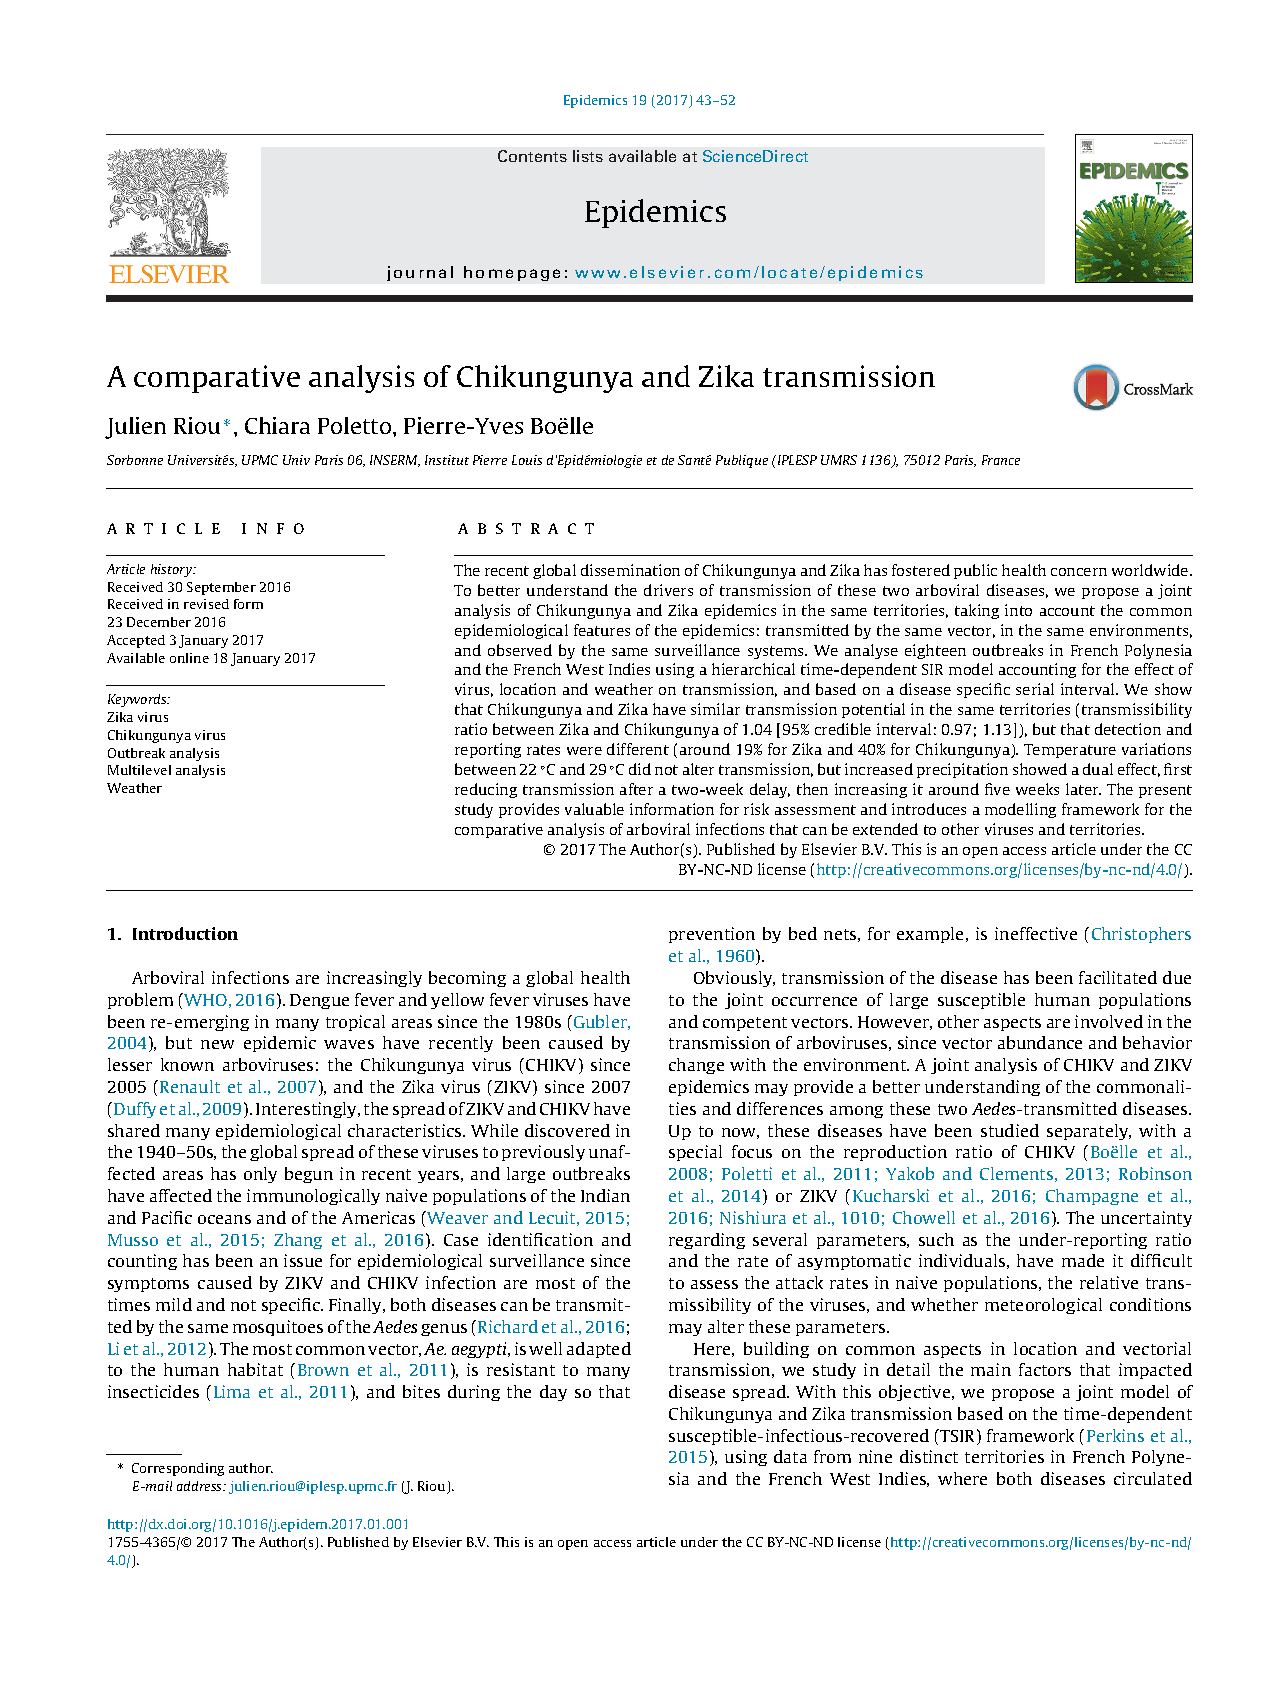
\includepdf[pages={1-10}]{Articles/epidemics.pdf}


\section{Principaux résultats}

Le modèle hiérarchique utilisé dans cette étude, intégrant les effets respectifs du virus, du territoire et des conditions météorologiques, permet d'obtenir une bonne description des dynamiques épidémiques observées lors de la circulation du chikungunya et du Zika en Polynésie française et aux Antilles françaises.
Les résultats répondent aux objectifs fixés :
\begin{itemize}
\item[(1)] Lorsque deux épidémies de chikungunya et de Zika surviennent successivement dans territoire \guillemotleft typique\guillemotright\ des régions étudiées, on s'attend à retrouver des niveaux de transmissibilité équivalents ($\beta_D=1,04$ ; intervalle de crédibilité à 95\% 0,97-1,13) mais un taux de signalement plus faible pour le Zika ($\omega=0,37$ ; IC95\% 0,34-0,40).
Cela correspond à des estimations de $\mathcal{R}_0$ moyennes toutes îles confondues de 1,82 (IC95\% 1,52-2,17) pour le chikungunya et de 1,87 (IC95\% 1,55-2,24) pour le Zika, un peu plus basses mais comparables à d'autres études sur le chikungunya ou le Zika dans les mêmes territoires \cite{kucharski2016transmission,Champagne064949,cauchemez2014local,nishiura2016transmission}, même si les différences d'approche méthodologique rendent la comparaison directe difficile.
Les estimations du taux de signalement sont de 41\% (IC95\% 29-55) pour le chikungunya et de 19\% (IC95\% 12-29) pour le Zika, ce qui est cohérent avec les différences connues entre les deux maladies concernant la proportion de cas symptomatiques (estimée à environ 30\% pour le Zika contre 80\% pour le chikungunya). 
D'autre part, cela suggère que les différences entre virus pouvant avoir une influence sur la transmissibilité, comme par exemple la probabilité de transmission par piqûre, n'ont que peu d'effet comparativement à d'autres facteurs liés aux vecteurs et aux hôtes.
\vspace{.3em}
\item[(2)] La température locale moyenne dans les huit semaines précédentes ne semble pas avoir influencé les niveaux de transmission durant les épidémies. Toutefois, la température est restée globalement stable durant ces épidémies, presque constamment entre 25 et 28$^{\circ}$C, et seulement un peu plus faible aux îles Australes, ce qui pourrait expliquer l'absence d'effet détecté contrairement à d'autres études \cite{li_rainfall_1985,barrera_population_2011,lu_time_2009}. Au contraire, on retrouve un effet sensible des précipitations sur la transmission : après la pluie, les niveaux de transmission diminuent d'environ 20\% pendant une à deux semaines ($\beta_{T,2}=0,81$ ; IC95\% 0,66-0,98), puis sont accrus après un délai de quatre à six semaines d'environ 30\% ($\beta_{T,5}=1,30$ ; IC95\% 1,09-1,56). Ce délai de quatre à six semaines est intéressant car il correspond au temps de développement des moustiques du stade larvaire au stade adulte \cite{barrera_population_2011}, ce qui fournit une interprétation plausible de ce résultat.
\vspace{.3em}
\item[(3)] L'estimation des paramètres de variance inter-île montrent une hétérogénéité résiduelle marquée de la transmissibilité et du taux de signalement. 
D'autres études ont aussi retrouvé des différences entre territoires \cite{kucharski2016transmission,Champagne064949,cauchemez2014local,nishiura2016transmission,chowell_using_2016,funk2016comparative}. 
Le modèle permet d'attribuer cette hétérogénéité aux caractéristiques spécifiques des îles, mais il est difficile d'aller au delà avec les données disponibles.
On observe une plus faible transmissibilité aux Antilles qu'en Polynésie, ce qui pourrait s'expliquer par des différences de population, d'environnement ou encore d'abondance et de composition des populations de vecteurs.
En particulier, le vecteur {\em Ae. polynesiensis}, présent seulement en Polynésie, a été considéré comme un vecteur possible de chikungunya et de Zika \cite{richard2016vector}.
Concernant le taux de signalement, il est probable que l'hétérogénéité soit liée à des différences d'organisation du système de soin et de surveillance. 
On observe d'ailleurs une tendance à des taux de signalement plus élevés dans les îles les moins peuplées, comme les îles Australes, les îles Marquises ou Saint-Martin.
Les taux de signalement sont aussi plus faibles en Martinique, sans qu'il existe d'explication évidente.
Des données plus précises, par exemple de type longitudinales, permettraient d'aller plus loin dans l'explication de ces différences et d'estimer l'influence de certains aspects comme par exemple la mobilité humaine \cite{stoddard2013house}, la qualité des habitations \cite{reiter_texas_2003}, ou encore le mode de gestion de l'eau et des ordures \cite{monath1994dengue}.

\end{itemize}

\section{Commentaires et perspectives}

Dans ce travail, nous avons développé un modèle hiérarchique innovant permettant l'analyse conjointe d'épidémies successives de chikungunya et de Zika dans neuf zones, quantifiant les effets respectifs du virus, des conditions météorologiques et du territoire sur les dynamiques de transmission et de surveillance.
Cela a permis de montrer les niveaux de transmission observés de ces épidémies dépendent peu du virus en cause, mais sont influencés par les conditions météorologiques, en particulier les précipitations.
Une large part de la variabilité entre les îles est liée à des caractéristiques locales, non-observées ici.
D'autres études utilisant des données plus détaillées pourraient permettre de mieux comprendre quelles sont les caractéristiques locales les plus influentes, ce qui pourrait mener à l'identification de nouvelles cibles d'action pour la prévention et le contrôle de ces maladies.
Ces résultats reposent toutefois sur plusieurs hypothèses limitantes, en particulier une part d'incertitude dans la construction mécaniste de l'intervalle de génération.

Pour autant, cette étude fournit des informations importantes.
Le fait que des épidémies successives de chikungunya et de Zika aient des niveaux de transmissibilité équivalents, mais des taux de signalement différents en lien avec la proportion de cas symptomatiques spécifique à chaque maladie est un résultat attendu, qu'il fallait pourtant démontrer et quantifier.
Des conclusions assez proches ont d'ailleurs été retrouvées dans une comparaison des épidémies de Zika et de dengue sur l'île de Yap \cite{funk2016comparative}.
De façon générale, les études d'épidémiologie comparée restent rares.
Par exemple, un travail a indiqué un coefficient de corrélation de 0,62 entre les nombres de reproductions de vagues successives de grippe aux \'Etats-Unis d'Amérique en 1889 et 1918 \cite{valleron2010transmissibility}.
Pourtant, l'extension de ce type de travail permet d'améliorer la compréhension des liens entre épidémies, et donc de certaines caractéristiques générales.
Cela pourrait avoir un effet bénéfique sur la préparation de la communauté internationale en cas de nouvelle émergence, en particulier de maladies transmises par les moustiques du genre {\em Aedes}.

\chapter{Épidémiologie prédictive}
\chaptermark{}

Nous avons souligné dans le premier chapitre l'importance des maladies transmises par les moustiques du genre {\em Aedes} pour la santé globale, et la très probable persistance de ce problème dans le futur.
La répartition actuelle des moustiques {\em Ae. aegypti} et {\em Ae. albopictus} est même susceptible de s'étendre avec les changements climatiques en cours.
Un des scénarios plausibles à moyen terme consiste en l'émergence explosive dans les populations humaines entièrement susceptibles d'un virus connu, mais à l'heure actuelle limité à un cycle enzootique dans une zone géographique restreinte, suivant les exemples récents du chikungunya et du Zika.
Nous avons présenté une liste non-exhaustive de virus répondant à ces critères au paragraphe \ref{sec:emerg}.

Lorsqu'une émergence survient, l'évaluation épidémiologique empirique en temps réel est utile pour aider les autorités de santé publique dans leur prise de décision.
Se basant généralement sur des modèles mathématiques utilisant les données d'incidence disponibles, cette évaluation consiste en l'estimation de paramètres comme le nombre de reproduction de base, et présente parfois des prédictions concernant par exemple le nombre total de cas attendus durant la totalité de l'épidémie ou la date du pic d'incidence.
Toutefois, ce type de travail se heurte souvent à une contradiction : pour être utile, il doit survenir tôt dans l'épidémie, afin d'être en mesure de guider efficacement la mise en place de mesures de prévention et de contrôle.
Pour autant, plus on se place tôt dans une épidémie, plus les données disponibles sont rares, et donc plus l'incertitude sur les estimations et les prédictions sont grandes.
En particulier, il a été montré qu'avant que le pic d'incidence soit observé, les prédictions sont limitées par la difficulté à estimer le taux de signalement \cite{heesterbeek2015modeling}.
Nous proposons ici une approche originale pour limiter cette incertitude, basée sur les informations disponibles sur des épidémies antérieures et similaires à l'épidémie d'intérêt.

\section{Présentation de l'étude}

Notre travail comparant les épidémies successives de chikungunya et de Zika, présenté au chapitre 3, a permis de quantifier les similarités et les différences entre les dynamiques épidémiques de ces maladies quand elles circulent dans un lieu donné.
Suivant cette logique, l'information concernant la dynamique d'une maladie dans un lieu donné pourrait donc être utilisée pour l'autre.
Dans ce travail, nous présentons une application de cette idée aux épidémies de Zika aux Antilles françaises, les dernières chronologiquement parmi les données disponibles utilisées au chapitre précédent et présentées dans la figure \ref{fig:profiles}.
En produisant rétrospectivement des prédictions à différents stades de ces épidémies, nous mesurons les avantages apportés en termes de fiabilité de prédiction par l'utilisation d'informations existantes à ce moment là sur les épidémies antérieures de chikungunya dans les mêmes territoires, ainsi que sur les épidémies successives de chikungunya et de Zika survenues en Polynésie française.

\subsection{Objectifs et stratégie d'analyse}

Considérons les données disponibles sur l'incidence observée les épidémies de Zika en Guadeloupe, en Martinique et à Saint-Martin de décembre 2015 à mars 2017 (jeu de données $\mathcal{D}1$, Fig. \ref{fig:preddata}).
\begin{figure}[t]
	\centering
	\includegraphics[width=15.5cm]{Figures/preddata.pdf}
	\caption{Incidence hebdomadaire lors des épidémies de Zika dans trois îles des Antilles françaises entre 2015 et 2017. Les lettres $S$ et $E$ désignent le début et la fin de la période de circulation autochtone intense (selon les définitions locales), et la lettre $P$ désigne la date du pic d'incidence (sources : {\em CIRE Antille-Guyane}).}
	\label{fig:preddata}
\end{figure}
Pour chaque date $K$ dans cet intervalle et dans chaque île séparément, un modèle de type TSIR, proche de celui adapté à une épidémie dans une île présenté au chapitre \ref{sec:tsir}, est ajusté aux données d'incidence disponibles {\em jusqu'à cette date}.
On obtient les distributions postérieures des paramètres du modèle : le paramètre de transmission $\beta_Z$ (ou de façon équivalente dans ce cas, $\mathcal{R}_{0,Z}$, $Z$ pour Zika), le paramètre de signalement $\rho_Z$ et le paramètre de surdispersion $\phi_Z$.
Les distributions a priori attribuées à ces paramètres sont non-informatives, ce qui implique que les estimations obtenues ne dépendent que des données d'incidence jusqu'à la date $K$. 
A partir de ces distributions postérieures, on simule le reste de l'épidémie de façon stochastique, obtenant des prédictions de l'incidence hebdomadaire de la semaine $K$ à la semaine $K+104$, que l'on peut ensuite confronter avec les vraies observations.
La qualité d'une prédiction est mesurée grâce à deux composants : la {\em précision} (la distance entre la prédiction moyenne et l'observation) et l'{\em acuité} (l'incertitude sur la prédiction).
Ces prédictions d'incidence hebdomadaire pouvaient aussi être transformées en d'autres indicateurs plus parlants et directement comparable avec les données observées durant l'épidémie, comme la taille finale de l'épidémie, l'incidence maximale attendue, la date du pic d'incidence ou la date de la fin de la période de circulation autochtone intense.

L'objectif est de comparer la qualité de ces prédictions à celle obtenue à la même date $K$ en utilisant en plus l'information issue des épidémies du passé dont les données sont disponibles.
Cette information est obtenue en analysant les épidémies passées avec un modèle hiérarchique, et introduite dans les modèle de prédiction en modifiant les distributions a priori des paramètres $\mathcal{R}_{0,Z}$ et $\rho_Z$.
Les distributions a priori sont construites de la manière suivante :

\begin{itemize}
\item les données concernant les épidémies de chikungunya dans les mêmes îles (jeu de données $\mathcal{D}2$), deux ans auparavant, permettent d'obtenir les distributions postérieures de $\mathcal{R}_{0,C}|\mathcal{D}2$ et $\rho_C|\mathcal{D}2$ ($C$ pour chikungunya) ;
\item les données concernant les épidémies successives de chikungunya et de Zika en Polynésie française (jeu de données $\mathcal{D}3$) permettent d'obtenir les distributions postérieures de $\beta_D|\mathcal{D}3$ et $\omega|\mathcal{D}2$, c'est à dire respectivement du ratio des paramètres de transmission du Zika par rapport au chikungunya, et l'odds-ratio des paramètres de signalement du Zika par rapport au chikungunya, si on conserve les notations introduites au paragraphe \ref{sec:presenttsir} ;
\item les distributions {\em a priori} attribuées à  $\mathcal{R}_{0,Z}$ et $\rho_Z$ sont alors obtenues en combinant deux à deux les distributions postérieures précédentes :
\begin{equation}
\mathcal{R}_{0,Z}|\mathcal{D}2,\mathcal{D}3 = \mathcal{R}_{0,C}|\mathcal{D}2 \times \beta_D|\mathcal{D}3
\end{equation}
\begin{equation}
\rho_Z|\mathcal{D}2,\mathcal{D}3 = \rho_C|\mathcal{D}2 \times \omega|\mathcal{D}2
\end{equation}
\end{itemize}

En d'autres termes, $\mathcal{R}_{0,Z}|\mathcal{D}2,\mathcal{D}3$ et $\rho_Z|\mathcal{D}2,\mathcal{D}3$ sont une expression de la valeur attendue pour $\mathcal{R}_{0,Z}$ et $\rho_Z$ pour une épidémie de Zika dans une île des Antilles sachant ce qui a été observé durant l'épidémie de chikungunya {\em dans cette même île} et durant les épidémies de Polynésie.
Ces distributions a priori sont donc qualifiées de \guillemotleft locales\guillemotright.
Alternativement, nous avons aussi utilisé des distributions a priori \guillemotleft régionales\guillemotright, obtenues de façon similaires mais basées sur les distribution des hyperparamètres régissant la structure hiérarchique des modèles utilisés, et donc pouvant être utilisées pour n'importe quelle île de la région présentant des caractéristiques similaires aux îles ici étudiées.



\section[Article 2]{Article 2 : \guillemotleft Improving early epidemiological assessment of emerging {\em Aedes}-transmitted epidemics using historical data\guillemotright}
\cleardoublepage
\includepdf[pages={1-16}]{Articles/plosntd3.pdf}
\cleardoublepage
%\includepdf[pages={1-22}]{Articles/plosntd2.pdf}

\section{Principaux résultats}

Cette étude indique qu'il est possible d'améliorer sensiblement la fiabilité des prédictions épidémiques précoces en situation d'émergence de Zika en prenant en compte l'information issue d'autres épidémies similaires de Zika et de chikungunya ayant eu lieu dans le passé.
Jusqu'à ce que le pic d'incidence soit atteint, les prédictions réalisées en utilisant des distributions a priori informatives avaient systématiquement une meilleure précision et une meilleure acuité.
Logiquement, les distributions locales, plus spécifiques, amenaient à de meilleurs résultats que les distributions régionales.
Plus concrètement, les prédictions réalisées précocement sans information a priori aboutissaient en moyenne à surestimer la taille finale de l'épidémie d'un facteur 3,3 (de 0,2 à 5,8) et l'incidence maximale de l'épidémie d'un facteur 15,3 (de 2,0 à 63,1).
Par contraste, l'utilisation des distribution a priori locales permettait d'obtenir des prédictions en moyenne 1,1 fois trop élevée (de 0,4 à 1,5) pour la taille épidémique finale, et 2,4 fois trop élevées (de 1,3 à 3,9) pour l'incidence maximale. 
L'amélioration apportée par les données historiques était moins claire concernant les prédictions de la date du pic d'incidence ou de la date de fin de la période de circulation autochtone intense.

\section{Commentaires et perspectives}

Prédire les conséquences d'une épidémie émergente dès son stade précoce est difficile.
Cette étude explore une approche basée sur l'utilisation d'informations pré-existantes pour améliorer la qualité de ces prédictions.
Les épidémies successives de chikungunya et de Zika dans les Antilles procurent un cas d'étude particulièrement favorable, avec des épidémies rapprochées, survenant dans les mêmes zones, et causées par des maladies partageant de nombreuses similitudes.
Les relations proches entre ces épidémies ont d'ailleurs été mises en évidence dans l'étude présentée au chapitre 3, suggérant qu'il est possible d'utiliser les informations obtenues sur les dynamiques épidémiques d'une épidémie pour aider à la prédiction de l'autre, un concept appelé {\em transportabilité} \cite{pearl2014external}.

Pour autant, l'amélioration de la qualité des prédictions est très sensible, montrant le potentiel de la méthodologie proposée, basée sur l'utilisation de modèles hiérarchiques et de distributions a priori informatives.
En effet, les modèles hiérarchiques sont particulièrement adaptés aux tâches de prédiction, car ils permettent de mettre en commun l'information provenant de plusieurs épidémies, et de capturer la variabilité existant à l'intérieur d'une localité, et celle existant entre les localités \cite{gelman2006multilevel}.
D'autre part, l'utilisation de distributions a priori informatives, et plus généralement des statistiques Bayésiennes, est appropriée pour ce travail qui repose en partie sur la gestion de l'incertitude. 

Alors que la prédiction précoces des conséquences des épidémies émergentes suscite de plus en plus d'intérêt, comme le montrent les récent concours mis en place pour la prédiction de la grippe \cite{flu2017}, d'Ebola \cite{viboud2017rapidd} ou du chikungunya \cite{darpa2014}, ce travail démontre que mieux comprendre les épidémies du passé et leurs relations peut mener concrètement à de meilleures prédiction, et donc à une meilleure préparation face aux émergences à venir.
Dans ce contexte, il est important de soutenir les travaux systématiques de documentation et d'analyse des épidémies passées \cite{tycho_nejm_2013}, ainsi que les travaux encore rares d'épidémiologie comparée.
Plus prosaïquement, notre approche et son application au chikungunya et au Zika pourrait s'avérer directement utile en cas de nouvelle émergence de maladie transmise par les moustiques du genre {\em Aedes}, une fois que la transportabilité des informations entre ces trois maladies aura pu être établie.


\chapter*{Conclusions}
\chaptermark{Conclusions}
\addcontentsline{toc}{chapter}{Conclusions}

Lorem ipsum



\backmatter
\singlespacing

\bibliography{biblio}
\bibliographystyle{unsrt}

\begin{appendices}
\chapter{Annexe A : Informations complémentaires à l'article 1}
\includepdf[pages={1-16}]{Articles/epidemics2.pdf}
\chapter{Annexe B : Informations complémentaires à l'article 2}
\includepdf[pages={1-22}]{Articles/plosntd2.pdf}
\end{appendices}



\end{document}
